%----------------------------------------------------------------------------------------------------------------------------
\graphicspath{{Parti/P04-Travi_rigide/C06-Telai_piani/Figure/}}
\chapter{Telai piani}
\label{cap:telai_piani}
%----------------------------------------------------------------------------------------------------------------------------

\begin{sommario}
	Si analizzano i telai piani, sistemi di travi con
	connessioni esclusivamente rigide che formano una
	o più maglie chiuse. Si introduce la doppia lettura
	topologica --- travi come corpi rigidi o nodi come
	protagonisti --- e se ne ricava la formula delle
	maglie come misura dell'iperstaticità interna.
	Si distingue l'iperstaticità interna da quella
	esterna e si discutono le strutture miste con
	elementi di molteplicità diversa.
	Si sviluppano le equazioni esplicite della seconda
	lettura: le condizioni di compatibilità nodale e
	le equazioni di equilibrio nodale con $N$, $T$, $M$
	come incognite, mettendone in luce la struttura
	duale $\bm{B} = \bm{A}^\top$.
	Si presenta la struttura parametrica della soluzione
	iperstatica per sovrapposizione, illustrata
	sull'esempio del portale doppiamente incastrato.
	La determinazione delle incognite iperstatiche
	$\chi_j$ richiede le condizioni di congruenza
	elastica ed è rinviata al Vol.~II.
\end{sommario}




%----------------------------------------------------------------------------------------------------------------------------
\section*{Considerazioni introduttive}
\label{sec:raccordo_telai}
%----------------------------------------------------------------------------------------------------------------------------

Nel \CAPref{cap:assemblaggi_travi} il catalogo delle
tipologie strutturali ha distinto i sistemi a
\emph{connessioni eterogenee} --- nei quali coesistono
nodi rigidi, cerniere interne e carrelli --- dai sistemi
a \emph{connessioni omogenee}, caratterizzati da un unico
tipo di connessione. Tra questi ultimi, i sistemi
reticolari --- connessioni esclusivamente a cerniera ---
sono stati sviluppati in dettaglio nel
\CAPref{cap:reticolari}. I \emph{telai}\index{telaio|textbf} costituiscono
l'altra famiglia omogenea: connessioni esclusivamente
rigide, che trasmettono integralmente forza normale,
taglio e momento flettente.

La caratteristica topologica che distingue i telai da
tutti i sistemi già incontrati è la presenza di
\emph{maglie chiuse}\index{maglia chiusa} con connessioni rigide. Questa
proprietà non è accidentale --- come nei sistemi
reticolari iperstatici, dove le aste ridondanti possono
essere rimosse preservando l'isostaticità --- ma è
\emph{intrinseca} alla tipologia: ogni maglia chiusa
contribuisce con tre gradi di iperstaticità interna,
indipendentemente dal numero e dalla disposizione dei
carichi. Un telaio non è analizzabile rimuovendo le
ridondanze senza alterarne la natura strutturale.

Questa iperstaticità intrinseca\index{iperstaticita@iperstaticità!intrinseca} ha una conseguenza
diretta sulla strategia di analisi: la distribuzione
degli sforzi interni non è determinabile dal solo
equilibrio, ma richiede le relazioni costitutive e
le condizioni di congruenza elastica. Il presente
capitolo costruisce i fondamenti topologici necessari
--- la doppia lettura, la formula delle maglie,
le equazioni esplicite della seconda lettura ---
che costituiscono il punto di partenza per la
trattazione completa dei telai nel Vol.~II.


%----------------------------------------------------------------------------------------------------------------------------
\section{La doppia lettura topologica}
\label{sec:telai_doppia_lettura}
%----------------------------------------------------------------------------------------------------------------------------

Nei sistemi reticolari i punti di connessione
sono \emph{nodi a cerniera} --- punti geometrici
senza rotazione propria. Nei telai i punti di
connessione sono invece \emph{nodi incastro}\index{nodo!incastro|textbf}:
la connessione rigida trasmette integralmente
tutte e tre le componenti di spostamento
generalizzato --- due traslazioni e una rotazione
--- e la rotazione diventa pertanto un grado di
libertà autonomo di ciascun nodo. Anche per i
telai la struttura ammette due letture duali
complementari:

\begin{itemize}[noitemsep]
	\item \emph{Prima lettura --- travi come corpi
		rigidi}: le travi sono i protagonisti, i nodi
	incastro sono i connettori. Ogni trave contribuisce
	con $n = 3$ gradi di libertà (due traslazioni e
	una rotazione); ogni nodo incastro tra $e_i$ travi
	convergenti impone $m_i = 3(e_i - 1)$ equazioni
	di congruenza (continuità completa di tutte e tre
	le componenti di spostamento generalizzato).
	Per dualità $\bm{B} = \bm{A}^\top$, il problema
	statico ha come variabili le reazioni dei nodi
	incastro interni --- $3(e_i-1)$ componenti per
	ciascun nodo con $e_i$ travi convergenti, pari
	alla molteplicità del collegamento --- e le
	reazioni dei vincoli esterni, con le equazioni
	di equilibrio delle singole travi come equazioni
	duali delle condizioni di congruenza (si veda il \PARref{sec:telai_equazioni}).
	
	
	\item \emph{Seconda lettura --- nodi come
		protagonisti}: i nodi incastro sono i protagonisti,
	le travi sono i vincoli. Ogni nodo incastro
	possiede $3$ gradi di libertà (due traslazioni
	e una rotazione, tutte trasmesse integralmente
	attraverso le connessioni rigide); ogni trave
	che connette due nodi impone $3$ condizioni di
	congruenza --- continuità delle due traslazioni
	e della rotazione tra i nodi di estremità.
	Per dualità, il problema statico ha come variabili
	le caratteristiche della sollecitazione nelle
	travi --- forza normale, taglio e momento alle
	estremità --- e le reazioni vincolari esterne,
	con le equazioni di equilibrio nodale come
	equazioni duali (si veda il \PARref{sec:telai_equazioni}).
\end{itemize}

\begin{oss}
	Nei sistemi reticolari la rotazione di ogni asta
	è univocamente determinata dalle posizioni dei due
	nodi di estremità e non costituisce un grado di
	libertà indipendente del sistema
	(\OSSref{oss:rotazione_asta} del
	\CAPref{cap:reticolari}). Nei telai la situazione
	è opposta: la connessione rigida trasmette
	integralmente la rotazione nodale, che diventa
	pertanto una variabile cinematica autonoma di
	ciascun nodo. Questa differenza si riflette
	direttamente nel numero di gradi di libertà
	nodali --- $2$ per i nodi a cerniera dei
	reticolari, $3$ per i nodi incastro dei telai
	--- e nella struttura delle equazioni della
	seconda lettura sviluppate nel
	\PARref{sec:telai_equazioni}.
\end{oss}


\section{Formula delle maglie e fonti di sovradeterminazione}
\label{sec:telai_formula_maglie}


Le due letture topologiche sono algebricamente
equivalenti e conducono allo stesso indice di
classificazione $\nu$. Nella prima lettura si
applica la formula generale dei sistemi di corpi
rigidi:
\[
\nu = 3n_e - m_{\text{int}} - m_{\text{est}},
\]
dove $m_{\text{int}}$ è la molteplicità complessiva
dei nodi incastro interni.

Nella seconda lettura, con $n_n$ nodi incastro
e $n_e$ travi, il numero complessivo di gradi di
libertà è $3n_n$ e ogni trave impone $3$ condizioni
di congruenza, per un totale di $3n_e$ vincoli
interni. Per un sistema connesso, i vincoli interni
necessari a ridurre i $3n_n$ gradi di libertà nodali
ai soli $3$ moti rigidi d'insieme sono $3(n_n - 1)$:
i vincoli interni in eccesso --- quelli che generano
iperstaticità interna --- sono pertanto:
\[
g_{\mathscr{i}}^{\text{int}}
= 3n_e - 3(n_n - 1)
= 3(n_e - n_n + 1)
= 3p,
\]
dove $p = n_e - n_n + 1$\index{formula delle maglie|textbf} è il numero ciclomatico\index{numero ciclomatico|textbf}
del grafo interno, ossia il numero di maglie chiuse
indipendenti. Le maglie emergono quindi come
conseguenza naturale della topologia del grafo:
ogni maglia chiusa corrisponde a una trave in
eccesso rispetto alla struttura ad albero minimale
($p = 0$, $n_e = n_n - 1$) e contribuisce con
$3$ gradi di iperstaticità interna.

Il grado di iperstaticità globale è:
\begin{equation}\label{eq:class_telaio_globale}
	g_i = g_{\mathscr{i}}^{\text{est}} +
	g_{\mathscr{i}}^{\text{int}}
	= (m_{\text{est}} - 3) + 3p.
\end{equation}

La \FIGref{fig:telai} illustra tre configurazioni
di telaio con numero crescente di maglie chiuse
e consente di verificare l'equivalenza delle due
formule. Per ciascuna configurazione i vincoli
esterni sono due incastri alla base
($m_{\text{est}} = 6$, $g_{\mathscr{i}}^{\text{est}} = 3$)
e il grado di iperstaticità globale è $g_i = 3 + 3p$.

Si verifica l'equivalenza delle due letture per
il portale a due piani ($p = 1$, sinistra).

\medskip
\noindent\textit{Prima lettura.}
Con $n_e = 6$ travi il totale dei gradi di libertà
è $3 \times 6 = 18$. La molteplicità interna si
calcola nodo per nodo: i nodi $3$ e $4$, in cui
convergono tre travi (colonna inferiore, colonna
superiore e traverso), contribuiscono ciascuno con
$m_i = 3(3-1) = 6$; i nodi $5$ e $6$, in cui
convergono due travi (colonna superiore e traverso
di sommità), contribuiscono ciascuno con
$m_i = 3(2-1) = 3$; la molteplicità interna totale
è $m_{\text{int}} = 6+6+3+3 = 18$. Il totale dei
vincoli è $m = m_{\text{int}} + m_{\text{est}}
= 18 + 6 = 24$:
\[
\nu = 3n_e - m = 18 - 24 = -6,
\quad g_i = 6. \quad\checkmark
\]


\noindent\textit{Seconda lettura.}
Con $n_n = 6$ nodi il totale dei gradi di libertà
è $3 \times 6 = 18$. Ogni trave impone $3$ condizioni
di congruenza, per un totale di $3n_e = 18$ vincoli
interni; il totale dei vincoli è
$m = 18 + 6 = 24$:
\[
\nu = 3n_n - m = 18 - 24 = -6,
\quad g_i = 6. \quad\checkmark
\]

Le due letture danno lo stesso risultato,
confermando la loro equivalenza algebrica.
Il grado di iperstaticità $g_i = 6$ corrisponde
al numero di tagli --- ciascuno di molteplicità $3$
--- necessari a ridurre il telaio a un sistema
di mensole isostatiche: due tagli, uno per ciascuna
trave orizzontale, liberano i due tronconi verticali
trasformandoli in mensole incastrate alla base.

%%%%%%%%%%%%%%%%%%%%%%%%%%%%%%%%%%%%%%%%%%%
\begin{figure}[htbp]
	\centering
	\begin{tikzpicture}[
		scale=0.85,
		trave/.style={line width=1.8pt, line cap=round,
			line join=round, black},
		etasta/.style={circle, draw=black, fill=white,
			inner sep=1pt, font=\scriptsize,
			line width=0.6pt},
		inc/.style={line width=1.2pt},
		]
		\draw[very thin, gray!40](3.8,-0.8)--(3.8,7.0);
		\draw[very thin, gray!40](8.2,-0.8)--(8.2,7.0);
		
		\def\h{1.6}
		
		%% ── PORTALE 1: 1 campata, 2 piani (p=1) ─────────────
		\coordinate(P1N1) at (0.5, 0);
		\coordinate(P1N2) at (2.5, 0);
		\coordinate(P1N3) at (0.5, \h);
		\coordinate(P1N4) at (2.5, \h);
		\coordinate(P1N5) at (0.5, 2*\h);
		\coordinate(P1N6) at (2.5, 2*\h);
		
		\draw[trave](P1N1)--(P1N3)--(P1N5);
		\draw[trave](P1N2)--(P1N4)--(P1N6);
		\draw[trave](P1N3)--(P1N4);
		\draw[trave](P1N5)--(P1N6);
		
		\draw[inc](P1N1)--++(-0.45,0)--++(0.90,0);
		\foreach \x in {-0.38,-0.20,-0.02,0.16,0.34}
		\draw[very thin]($(P1N1)+(\x,0)$)--++(-.14,-0.17);
		\draw[inc](P1N2)--++(-0.45,0)--++(0.90,0);
		\foreach \x in {-0.38,-0.20,-0.02,0.16,0.34}
		\draw[very thin]($(P1N2)+(\x,0)$)--++(-.14,-0.17);
		
		\node[above left, font=\scriptsize] at (P1N1){$1$};
		\node[above right,font=\scriptsize] at (P1N2){$2$};
		\node[left, font=\scriptsize] at (P1N3){$3$};
		\node[right,font=\scriptsize] at (P1N4){$4$};
		\node[left, font=\scriptsize] at (P1N5){$5$};
		\node[right,font=\scriptsize] at (P1N6){$6$};
		
		\node[etasta] at ($(P1N1)!0.5!(P1N3)+(-0.30,0)$){$1$};
		\node[etasta] at ($(P1N2)!0.5!(P1N4)+(0.30,0)$) {$2$};
		\node[etasta] at ($(P1N3)!0.5!(P1N4)+(0,0.25)$) {$3$};
		\node[etasta] at ($(P1N3)!0.5!(P1N5)+(-0.30,0)$){$4$};
		\node[etasta] at ($(P1N4)!0.5!(P1N6)+(0.30,0)$) {$5$};
		\node[etasta] at ($(P1N5)!0.5!(P1N6)+(0,0.25)$) {$6$};
		
		\node[font=\small,gray] at (1.5,-0.60){$p=1$};
		
		%% ── PORTALE 2: 1 campata, 3 piani (p=2) ─────────────
		\def\ox{4.5}
		
		\coordinate(P2N1) at (\ox+0, 0);
		\coordinate(P2N2) at (\ox+2, 0);
		\coordinate(P2N3) at (\ox+0,   \h);
		\coordinate(P2N4) at (\ox+2,   \h);
		\coordinate(P2N5) at (\ox+0, 2*\h);
		\coordinate(P2N6) at (\ox+2, 2*\h);
		\coordinate(P2N7) at (\ox+0, 3*\h);
		\coordinate(P2N8) at (\ox+2, 3*\h);
		
		\draw[trave](P2N1)--(P2N3)--(P2N5)--(P2N7);
		\draw[trave](P2N2)--(P2N4)--(P2N6)--(P2N8);
		\draw[trave](P2N3)--(P2N4);
		\draw[trave](P2N5)--(P2N6);
		\draw[trave](P2N7)--(P2N8);
		
		\draw[inc](P2N1)--++(-0.45,0)--++(0.90,0);
		\foreach \x in {-0.38,-0.20,-0.02,0.16,0.34}
		\draw[very thin]($(P2N1)+(\x,0)$)--++(-.14,-0.17);
		\draw[inc](P2N2)--++(-0.45,0)--++(0.90,0);
		\foreach \x in {-0.38,-0.20,-0.02,0.16,0.34}
		\draw[very thin]($(P2N2)+(\x,0)$)--++(-.14,-0.17);
		
		\node[above left, font=\scriptsize] at (P2N1){$1$};
		\node[above right,font=\scriptsize] at (P2N2){$2$};
		\node[left, font=\scriptsize] at (P2N3){$3$};
		\node[right,font=\scriptsize] at (P2N4){$4$};
		\node[left, font=\scriptsize] at (P2N5){$5$};
		\node[right,font=\scriptsize] at (P2N6){$6$};
		\node[left, font=\scriptsize] at (P2N7){$7$};
		\node[right,font=\scriptsize] at (P2N8){$8$};
		
		\node[etasta] at ($(\ox+0,0)!0.5!(\ox+0,\h)+(-0.30,0)$)    {$1$};
		\node[etasta] at ($(\ox+2,0)!0.5!(\ox+2,\h)+(0.30,0)$)     {$2$};
		\node[etasta] at ($(\ox+0,\h)!0.5!(\ox+2,\h)+(0,0.25)$)    {$3$};
		\node[etasta] at ($(\ox+0,\h)!0.5!(\ox+0,2*\h)+(-0.30,0)$) {$4$};
		\node[etasta] at ($(\ox+2,\h)!0.5!(\ox+2,2*\h)+(0.30,0)$)  {$5$};
		\node[etasta] at ($(\ox+0,2*\h)!0.5!(\ox+2,2*\h)+(0,0.25)$){$6$};
		\node[etasta] at ($(\ox+0,2*\h)!0.5!(\ox+0,3*\h)+(-0.30,0)$){$7$};
		\node[etasta] at ($(\ox+2,2*\h)!0.5!(\ox+2,3*\h)+(0.30,0)$){$8$};
		\node[etasta] at ($(\ox+0,3*\h)!0.5!(\ox+2,3*\h)+(0,0.25)$){$9$};
		
		\node[font=\small,gray] at (\ox+1,-0.60){$p=2$};
		
		%% ── PORTALE 3: 1 campata, 4 piani (p=3) ─────────────
		\def\oxx{9.0}
		
		\coordinate(P3N1)  at (\oxx+0, 0);
		\coordinate(P3N2)  at (\oxx+2, 0);
		\coordinate(P3N3)  at (\oxx+0,   \h);
		\coordinate(P3N4)  at (\oxx+2,   \h);
		\coordinate(P3N5)  at (\oxx+0, 2*\h);
		\coordinate(P3N6)  at (\oxx+2, 2*\h);
		\coordinate(P3N7)  at (\oxx+0, 3*\h);
		\coordinate(P3N8)  at (\oxx+2, 3*\h);
		\coordinate(P3N9)  at (\oxx+0, 4*\h);
		\coordinate(P3N10) at (\oxx+2, 4*\h);
		
		\draw[trave](P3N1)--(P3N3)--(P3N5)--(P3N7)--(P3N9);
		\draw[trave](P3N2)--(P3N4)--(P3N6)--(P3N8)--(P3N10);
		\draw[trave](P3N3)--(P3N4);
		\draw[trave](P3N5)--(P3N6);
		\draw[trave](P3N7)--(P3N8);
		\draw[trave](P3N9)--(P3N10);
		
		\draw[inc](P3N1)--++(-0.45,0)--++(0.90,0);
		\foreach \x in {-0.38,-0.20,-0.02,0.16,0.34}
		\draw[very thin]($(P3N1)+(\x,0)$)--++(-.14,-0.17);
		\draw[inc](P3N2)--++(-0.45,0)--++(0.90,0);
		\foreach \x in {-0.38,-0.20,-0.02,0.16,0.34}
		\draw[very thin]($(P3N2)+(\x,0)$)--++(-.14,-0.17);
		
		\node[above left, font=\scriptsize] at (P3N1) {$1$};
		\node[above right,font=\scriptsize] at (P3N2) {$2$};
		\node[left, font=\scriptsize] at (P3N3) {$3$};
		\node[right,font=\scriptsize] at (P3N4) {$4$};
		\node[left, font=\scriptsize] at (P3N5) {$5$};
		\node[right,font=\scriptsize] at (P3N6) {$6$};
		\node[left, font=\scriptsize] at (P3N7) {$7$};
		\node[right,font=\scriptsize] at (P3N8) {$8$};
		\node[left, font=\scriptsize] at (P3N9) {$9$};
		\node[right,font=\scriptsize] at (P3N10){$10$};
		
		\node[etasta] at ($(\oxx+0,0)!0.5!(\oxx+0,\h)+(-0.30,0)$)     {$1$};
		\node[etasta] at ($(\oxx+2,0)!0.5!(\oxx+2,\h)+(0.30,0)$)      {$2$};
		\node[etasta] at ($(\oxx+0,\h)!0.5!(\oxx+2,\h)+(0,0.25)$)     {$3$};
		\node[etasta] at ($(\oxx+0,\h)!0.5!(\oxx+0,2*\h)+(-0.30,0)$)  {$4$};
		\node[etasta] at ($(\oxx+2,\h)!0.5!(\oxx+2,2*\h)+(0.30,0)$)   {$5$};
		\node[etasta] at ($(\oxx+0,2*\h)!0.5!(\oxx+2,2*\h)+(0,0.25)$) {$6$};
		\node[etasta] at ($(\oxx+0,2*\h)!0.5!(\oxx+0,3*\h)+(-0.30,0)$){$7$};
		\node[etasta] at ($(\oxx+2,2*\h)!0.5!(\oxx+2,3*\h)+(0.30,0)$) {$8$};
		\node[etasta] at ($(\oxx+0,3*\h)!0.5!(\oxx+2,3*\h)+(0,0.25)$) {$9$};
		\node[etasta] at ($(\oxx+0,3*\h)!0.5!(\oxx+0,4*\h)+(-0.30,0)$){$10$};
		\node[etasta] at ($(\oxx+2,3*\h)!0.5!(\oxx+2,4*\h)+(0.30,0)$) {$11$};
		\node[etasta] at ($(\oxx+0,4*\h)!0.5!(\oxx+2,4*\h)+(0,0.25)$) {$12$};
		
		\node[font=\small,gray] at (\oxx+1,-0.60){$p=3$};
		
	\end{tikzpicture}
	\caption{Tre configurazioni di telaio piano a una
		campata: due piani ($p=1$, $n_e=6$, $n_n=6$,
		sinistra), tre piani ($p=2$, $n_e=9$, $n_n=8$,
		centro), quattro piani ($p=3$, $n_e=12$,
		$n_n=10$, destra). I vincoli esterni sono
		incastri alla base in tutti e tre i casi
		($m_{\text{est}}=6$, $g_{\mathscr{i}}^{\text{est}}=3$).
		Il grado di iperstaticità globale è
		$g = 3 + 3p$: rispettivamente $6$, $9$, $12$.
		I nodi sono numerati $1$--$n_n$, le aste
		con il numero cerchiato.}
	\label{fig:telai}
\end{figure}
%%%%%%%%%%%%%%%%%%%%%%%%%%%%%%%%%%%%%%%%%%%

\paragraph{Sovradeterminazione esterna.}
Il grado di sovradeterminazione esterna dipende
esclusivamente dai vincoli al suolo ed è indipendente
dalla topologia interna del telaio:
\begin{equation}\label{eq:g_est_telaio}
	g_i^{\text{est}} = m_{\text{est}} - 3,
\end{equation}
purché i vincoli esterni siano geometricamente
indipendenti. La sovradeterminazione esterna ha
le stesse conseguenze cinematiche già discusse
per i sistemi reticolari
(\SECref{sec:muller_breslau_classificazione}
del \CAPref{cap:reticolari}): i cedimenti
vincolari devono soddisfare $g_i^{\text{est}}$
condizioni di compatibilità e le reazioni al suolo
non sono univocamente determinate dall'equilibrio
globale.

\paragraph{Grado di iperstaticità totale.}
Il grado di iperstaticità globale si ottiene
sommando i due contributi:
\begin{equation}\label{eq:g_tot_telaio}
	g_i = g_i^{\text{est}} + g_i^{\text{int}}
	= (m_{\text{est}} - 3) + 3p.
\end{equation}
Le due fonti hanno conseguenze fisiche distinte
e non si sostituiscono a vicenda: la
sovradeterminazione interna rende la distribuzione
degli sforzi nelle travi dipendente dalla rigidezza
relativa degli elementi; quella esterna rende le
reazioni vincolari indeterminate dall'equilibrio.
Entrambe richiedono le condizioni di congruenza
elastica per la loro risoluzione, sviluppate
nel Vol.~II.

\paragraph{Comportamento esterno e interno.}
La distinzione tra iperstaticità esterna e interna
è particolarmente rilevante per i telai. Un telaio
può essere isostatico esternamente e iperstatico
internamente (appoggi semplici con maglie chiuse),
iperstatico sia esternamente che internamente
(incastri alla base con maglie chiuse), o isostatico
globalmente per opportuna combinazione di vincoli
e cerniere interne (portale a tre cerniere).
L'inserimento di una cerniera interna in un nodo
riduce $g_{\mathscr{i}}^{\text{int}}$ di una quantità
che dipende dalla valenza del nodo, come precisato
nell'osservazione che segue.
I problemi cinematico e statico dei telai ---
equazioni di compatibilità nodale, matrice di
rotazione e equazioni di equilibrio nodale ---
sono sviluppati nel \PARref{par:equazioni_seconda_lettura_telai}
del presente capitolo.

\begin{oss}
	L'inserimento di una cerniera interna in un
	nodo a $e_c$ vie riduce $g_{\mathscr{i}}^{\text{int}}$
	di $(e_c - 1)$, poiché rilascia $(e_c - 1)$
	condizioni di congruenza rotazionale --- una
	per ciascuna coppia di travi convergenti nel
	nodo. La formula generale per un telaio con
	$p$ maglie chiuse e cerniere interne nei nodi
	$c = 1, \ldots, n_c$ è pertanto:
	\begin{equation}\label{eq:gint_cerniere}
		g_{\mathscr{i}}^{\text{int}}
		= 3p - \sum_{c=1}^{n_c}(e_c - 1),
	\end{equation}
	purché le cerniere siano collocate in posizioni
	non degeneri. Il caso limite di una maglia con
	tre cerniere interne a due vie ($e_c = 2$,
	$\sum(e_c-1) = 3$) dà
	$g_{\mathscr{i}}^{\text{int}} = 0$: la maglia
	è chiusa ma internamente isostatica, come nel
	sistema a tre cerniere del catalogo.
\end{oss}


\begin{oss}[Dalla topologia del grafo interno
	alla formula delle maglie]
	Il conteggio delle maglie $p$ si applica al
	\emph{grafo interno} della struttura, formato
	dalle sole travi come spigoli e dai soli nodi
	incastro come vertici. I vincoli al suolo ---
	carrelli, cerniere, incastri --- sono vincoli
	\emph{esterni} e non entrano nel conteggio di
	$p$: essi contribuiscono separatamente alla
	molteplicità $m_\text{est}$.
	
	Per un grafo interno connesso con $n_e$ travi
	e $n_n$ nodi, il numero di maglie indipendenti
	--- detto \emph{numero ciclomatico} --- è dato
	dalla formula di Eulero:
	\begin{equation}\label{eq:eulero_grafo}
		p = n_e - n_n + 1.
	\end{equation}
	Un telaio con struttura interna ad albero
	($p = 0$, ossia $n_e = n_n - 1$) è internamente
	isostatico. Ogni trave aggiuntiva che chiude una
	maglia interna ($p \to p+1$) aggiunge $3$
	condizioni di compatibilità senza aggiungere
	gradi di libertà nodali, incrementando
	$g_{\mathscr{i}}^{\text{int}}$ di $3$, donde
	$g_{\mathscr{i}}^{\text{int}} = 3p = 3(n_e-n_n+1)$.
\end{oss}

\begin{oss}[Inclusione del suolo come elemento
	strutturale]
	Una descrizione alternativa, talvolta adottata,
	include il \emph{suolo} come elemento strutturale
	aggiuntivo che collega rigidamente i nodi di base.
	Per il portale a due piani ($p=1$), il suolo
	forma una settima trave che chiude un secondo
	rettangolo: $n_e = 7$, $n_n = 6$,
	$p = 7-6+1 = 2$, da cui
	$g_{\mathscr{i}}^{\text{int}} = 6$ e
	$g_{\mathscr{i}}^{\text{est}} = 0$.
	Le due descrizioni danno lo stesso grado totale
	$g = 6$, ma attribuiscono diversamente la
	ridondanza tra comportamento esterno e interno.
	La convenzione adottata in questo volume ---
	il suolo come ambiente esterno, non come elemento
	strutturale --- preserva la distinzione tra
	comportamento esterno e interno ed è coerente
	con l'approccio seguito per tutti gli altri
	sistemi di travi.
\end{oss}



%----------------------------------------------------------------------------------------------------------------------------
\section{Morfologia dei telai piani}
\label{sec:telai_morfologia}
%----------------------------------------------------------------------------------------------------------------------------

Nei telai piani si distinguono convenzionalmente
due gruppi di travi in base alla loro funzione
geometrica nel sistema:

\begin{itemize}
	\item le \emph{travi orizzontali}, dette anche
	\emph{traversi}\index{traverso|textbf} o \emph{correnti}, che collegano
	i montanti a uno stesso livello e trasferiscono
	i carichi verticali alle colonne;
	
	\item le \emph{travi verticali}, dette
	\emph{montanti} o \emph{colonne}\index{colonna|textbf}, che collegano
	i nodi di piani successivi e trasferiscono
	i carichi verticali alle fondazioni.
\end{itemize}

Questa ripartizione è puramente descrittiva e
dipende dall'orientamento prevalente del telaio:
nei telai inclinati o nei portici a geometria
irregolare la distinzione tra traversi e montanti
perde significato e si parla semplicemente di
\emph{travi di telaio}\index{trave!di telaio|textbf}.

Le configurazioni più comuni si classificano
in base al numero di campate orizzontali
$n_c$ e al numero di piani $n_p$\nomenclature[L]{$n_p$}{numero di piani del telaio}:

\begin{itemize}
	\item \emph{telaio a una campata}\index{telaio!a una campata|textbf} ($n_c = 1$):
	il portale\index{portale|textbf}, nella sua versione più semplice;
	
	\item \emph{telaio a più campate}\index{telaio!a più campate|textbf}
	($n_c \geq 2$): più portali affiancati,
	con montanti condivisi tra campate adiacenti;
	
	\item \emph{telaio a più piani}\index{telaio!a più piani|textbf}
	($n_p \geq 2$): portali sovrapposti,
	con traversi condivisi tra piani adiacenti.
\end{itemize}

In tutti i casi il numero di maglie chiuse
indipendenti è $p = n_c \cdot n_p$, da cui
il grado di iperstaticità interna
$g_i^{\text{int}} = 3n_c n_p$ per un telaio
con soli nodi rigidi interni e vincoli
esterni minimi ($m_{\text{est}} = 3$,
$g_i^{\text{est}} = 0$).



\paragraph{Strutture miste: cerniere interne nei telai.}
Le \emph{strutture miste}\index{struttura mista|textbf} combinano elementi di
molteplicità diversa nello stesso sistema: travi
di telaio ($m = 3$), travi con svincolo ($m = 2$)
e aste reticolari ($m = 1$) possono coesistere,
e la classificazione del sistema si ottiene
sommando i contributi di ciascun elemento secondo
la formula generale $\nu = 3n_e - m$.
Sul versante cinematico, nodi a cui convergono
elementi di molteplicità diversa ammettono
spostamenti relativi parziali --- alcune componenti
vincolate, altre libere --- con le corrispondenti
grandezze statiche trasmesse e non trasmesse.
La \FIGref{fig:strutture_miste} illustra tre
varianti di un portale a due piani in cui elementi
di molteplicità diversa coesistono nello stesso
sistema. In tutti e tre i casi il telaio di
partenza ha $g = 6$ ($g_{\mathscr{i}}^{\text{est}}
= 3$, $g_{\mathscr{i}}^{\text{int}} = 3$);
le modifiche introdotte riducono il grado di
iperstaticità in modo diverso a seconda della
natura e della posizione degli elementi introdotti.

\medskip
\noindent\textbf{Portale (A) --- cerniera interna
	nel nodo~$3$.}
Il nodo~$3$ è un nodo incastro a tre vie;
l'inserimento di una cerniera lo trasforma in
un nodo cerniera, rilasciando $e_3 - 1 = 2$
condizioni di congruenza rotazionale.
Nella prima lettura, con $n_e = 6$ travi:
\[
m_{\text{int}} = 4_{(3)} + 6_{(4)} +
3_{(5)} + 3_{(6)} = 16,
\quad
\nu = 3\times6 - 16 - 6 = -4,
\quad g = 4.
\]
Nella seconda lettura, con $5$ nodi incastro
e $1$ nodo cerniera:
\[
n = 3\times5 + 2\times1 = 17,
\quad
m_{\text{int}} = 15,
\quad
\nu = 17 - 21 = -4. \quad\checkmark
\]
La riduzione $g: 6 \to 4$ è interamente interna:
$g_{\mathscr{i}}^{\text{int}}$ passa da $3$ a $1$,
mentre $g_{\mathscr{i}}^{\text{est}} = 3$ rimane
invariato.

\medskip
\noindent\textbf{Portale (B) --- diagonale
	reticolare tra i nodi~$3$ e~$6$.}
La diagonale reticolare ($m = 1$) trasforma i
nodi~$3$ e~$6$ da nodi incastro a nodi cerniera.
Nella prima lettura, con $n_e = 7$ aste
($n = 21$):
\[
m_{\text{int}} = 6_{(3)} + 6_{(4)} +
3_{(5)} + 4_{(6)} = 19,
\quad
\nu = 3\times7 - 19 - 6 = -4,
\quad g = 4.
\]
Nella seconda lettura, con $4$ nodi incastro
e $2$ nodi cerniera:
\[
n = 3\times4 + 2\times2 = 16,
\quad
m_{\text{int}} = 14,
\quad
\nu = 16 - 20 = -4. \quad\checkmark
\]
Anche in questo caso $g: 6 \to 4$, ma per una
ragione diversa: non è rilasciata una condizione
rotazionale in un nodo incastro esistente, bensì
il nuovo collegamento ha molteplicità $m = 1$
invece di $m = 3$, e i due nodi alle sue estremità
perdono la continuità rotazionale.

\medskip
\noindent\textbf{Portale (C) --- cerniera in~$3$
	e diagonale reticolare tra i nodi~$5$ e~$4$.}
Le due modifiche coesistono: il nodo~$3$ diventa
nodo cerniera per effetto della cerniera interna,
i nodi~$4$ e~$5$ diventano nodi cerniera per
effetto della diagonale reticolare.
Nella prima lettura, con $n_e = 7$ aste
($n = 21$):
\[
m_{\text{int}} = 4_{(3)} + 6_{(4)} +
4_{(5)} + 3_{(6)} = 17,
\quad
\nu = 3\times7 - 17 - 6 = -2,
\quad g = 2.
\]
Nella seconda lettura, con $3$ nodi incastro
e $3$ nodi cerniera:
\[
n = 3\times3 + 2\times3 = 15,
\quad
m_{\text{int}} = 11,
\quad
\nu = 15 - 17 = -2. \quad\checkmark
\]
Le due modifiche interagiscono: la riduzione
complessiva $g: 6 \to 2$ è maggiore della somma
delle riduzioni individuali dei portali (A) e (B)
($\Delta g = 2$ ciascuno). Per i sistemi misti
la decomposizione $g = g_{\mathscr{i}}^{\text{est}}
+ g_{\mathscr{i}}^{\text{int}}$ non si applica
direttamente: la distinzione tra iperstaticità esterna e
interna richiede un'analisi specifica del sistema,
che sarà sviluppata nel Vol.~II nel contesto
dei metodi matriciali.


\begin{figure}[htbp]
	\centering
	\begin{tikzpicture}[
		scale=0.85,
		trave/.style={line width=1.8pt, line cap=round,
			line join=round, black},
		diag/.style={line width=1.8pt, line cap=round,
			line join=round, gray!60},
		nodoInc/.style={},
		nodoCer/.style={circle, fill=white, draw=black,
			inner sep=0pt, minimum size=4pt,
			line width=1.2pt},
		cerInt/.style={circle, fill=white,
			draw=black!60!orange,
			inner sep=0pt, minimum size=4pt,
			line width=1.5pt},
		inc/.style={line width=1.2pt},
		etasta/.style={circle, draw=black, fill=white,
			inner sep=1pt, font=\scriptsize,
			line width=0.6pt},
		]
		
		\def\h{1.6}
		\def\sep{4.5}
		
		%% ── separatori verticali ─────────────────────────────────
		\draw[very thin, gray!40](3.6,-0.8)--(3.6,4.5);
		\draw[very thin, gray!40](8.2,-0.8)--(8.2,4.5);
		
		%% ═══════════════════════════════════════════════════════
		%% PORTALE A — cerniera nel nodo 3 (tre vie)
		%% nodi: 1(0.5,0) 2(2.5,0) 3(0.5,h) 4(2.5,h)
		%%        5(0.5,2h) 6(2.5,2h)
		%% ═══════════════════════════════════════════════════════
		
		\coordinate(AN1) at (0.5, 0);
		\coordinate(AN2) at (2.5, 0);
		\coordinate(AN3) at (0.5, \h);
		\coordinate(AN4) at (2.5, \h);
		\coordinate(AN5) at (0.5, 2*\h);
		\coordinate(AN6) at (2.5, 2*\h);
		
		\draw[trave](AN1)--(AN3);
		\draw[trave](AN2)--(AN4);
		\draw[trave](AN3)--(AN4);
		\draw[trave](AN3)--(AN5);
		\draw[trave](AN4)--(AN6);
		\draw[trave](AN5)--(AN6);
		
		%% incastri
		\draw[inc](AN1)--++(-0.45,0)--++(0.90,0);
		\foreach \x in {-0.38,-0.20,-0.02,0.16,0.34}
		\draw[very thin]($(AN1)+(\x,0)$)--++(-.14,-0.17);
		\draw[inc](AN2)--++(-0.45,0)--++(0.90,0);
		\foreach \x in {-0.38,-0.20,-0.02,0.16,0.34}
		\draw[very thin]($(AN2)+(\x,0)$)--++(-.14,-0.17);
		
		%% cerniera interna nel nodo 3
		\node[nodoCer] at (AN3){};
		
		%% nodi incastro (nessun simbolo — travi continue)
		%% etichette nodi
		\node[above left, font=\scriptsize] at (AN1){$1$};
		\node[above right,font=\scriptsize] at (AN2){$2$};
		\node[left, font=\scriptsize]	at (AN3){$3$};
		\node[right,font=\scriptsize] at (AN4){$4$};
		\node[left, font=\scriptsize] at (AN5){$5$};
		\node[right,font=\scriptsize] at (AN6){$6$};
		
		%% numerazione aste
		\node[etasta] at ($(AN1)!0.5!(AN3)+(-0.30,0)$){$1$};
		\node[etasta] at ($(AN2)!0.5!(AN4)+(0.30,0)$) {$2$};
		\node[etasta] at ($(AN3)!0.5!(AN4)+(0,0.22)$) {$3$};
		\node[etasta] at ($(AN3)!0.5!(AN5)+(-0.30,0)$){$4$};
		\node[etasta] at ($(AN4)!0.5!(AN6)+(0.30,0)$) {$5$};
		\node[etasta] at ($(AN5)!0.5!(AN6)+(0,0.22)$) {$6$};
		
		\node[font=\small,gray] at (1.5,-0.60){$g=4$};
		
		%% ═══════════════════════════════════════════════════════
		%% PORTALE B — diagonale reticolare nodo 3 → nodo 6
		%% nodi: 1..6, offset x = sep
		%% ═══════════════════════════════════════════════════════
		
		\coordinate(BN1) at (\sep+0.5, 0);
		\coordinate(BN2) at (\sep+2.5, 0);
		\coordinate(BN3) at (\sep+0.5, \h);
		\coordinate(BN4) at (\sep+2.5, \h);
		\coordinate(BN5) at (\sep+0.5, 2*\h);
		\coordinate(BN6) at (\sep+2.5, 2*\h);
		
		\draw[trave](BN1)--(BN3);
		\draw[trave](BN2)--(BN4);
		\draw[trave](BN3)--(BN4);
		\draw[trave](BN3)--(BN5);
		\draw[trave](BN4)--(BN6);
		\draw[trave](BN5)--(BN6);
		%% diagonale reticolare (grigia)
		\draw[diag](BN3)--(BN6);
		
		%% incastri
		\draw[inc](BN1)--++(-0.45,0)--++(0.90,0);
		\foreach \x in {-0.38,-0.20,-0.02,0.16,0.34}
		\draw[very thin]($(BN1)+(\x,0)$)--++(-.14,-0.17);
		\draw[inc](BN2)--++(-0.45,0)--++(0.90,0);
		\foreach \x in {-0.38,-0.20,-0.02,0.16,0.34}
		\draw[very thin]($(BN2)+(\x,0)$)--++(-.14,-0.17);
		
		%% cerniere alle estremità della diagonale
		\node[nodoCer] at (BN3){};
		\node[nodoCer] at (BN6){};
		
		%% etichette nodi
		\node[above left, font=\scriptsize] at (BN1){$1$};
		\node[above right,font=\scriptsize] at (BN2){$2$};
		\node[left, font=\scriptsize] at (BN3){$3$};
		\node[right,font=\scriptsize] at (BN4){$4$};
		\node[left, font=\scriptsize] at (BN5){$5$};
		\node[right,font=\scriptsize] at (BN6){$6$};
		
		%% numerazione aste
		\node[etasta] at ($(\sep+0.5,0)!0.5!(\sep+0.5,\h)+(-0.30,0)$){$1$};
		\node[etasta] at ($(\sep+2.5,0)!0.5!(\sep+2.5,\h)+(0.30,0)$) {$2$};
		\node[etasta] at ($(\sep+0.5,\h)!0.5!(\sep+2.5,\h)+(0,0.22)$){$3$};
		\node[etasta] at ($(\sep+0.5,\h)!0.5!(\sep+0.5,2*\h)+(-0.30,0)$){$4$};
		\node[etasta] at ($(\sep+2.5,\h)!0.5!(\sep+2.5,2*\h)+(0.30,0)$){$5$};
		\node[etasta] at ($(\sep+0.5,2*\h)!0.5!(\sep+2.5,2*\h)+(0,0.22)$){$6$};
		%% diagonale: etichetta a metà
		\node[etasta] at ($(\sep+0.5,\h)!0.5!(\sep+2.5,2*\h)+(0.35,0)$){$7$};
		
		\node[font=\small,gray] at (\sep+1.5,-0.60){$g=4$};
		
		%% ═══════════════════════════════════════════════════════
		%% PORTALE C — cerniera in 3 + diagonale 5 → 4
		%% nodi: 1..6, offset x = 2*sep
		%% ═══════════════════════════════════════════════════════
		
		\def\secc{9.0}
		
		\coordinate(CN1) at (\secc+0.5, 0);
		\coordinate(CN2) at (\secc+2.5, 0);
		\coordinate(CN3) at (\secc+0.5, \h);
		\coordinate(CN4) at (\secc+2.5, \h);
		\coordinate(CN5) at (\secc+0.5, 2*\h);
		\coordinate(CN6) at (\secc+2.5, 2*\h);
		
		\draw[trave](CN1)--(CN3);
		\draw[trave](CN2)--(CN4);
		\draw[trave](CN3)--(CN4);
		\draw[trave](CN3)--(CN5);
		\draw[trave](CN4)--(CN6);
		\draw[trave](CN5)--(CN6);
		%% diagonale reticolare 5→4 (grigia)
		\draw[diag](CN5)--(CN4);
		
		%% incastri
		\draw[inc](CN1)--++(-0.45,0)--++(0.90,0);
		\foreach \x in {-0.38,-0.20,-0.02,0.16,0.34}
		\draw[very thin]($(CN1)+(\x,0)$)--++(-.14,-0.17);
		\draw[inc](CN2)--++(-0.45,0)--++(0.90,0);
		\foreach \x in {-0.38,-0.20,-0.02,0.16,0.34}
		\draw[very thin]($(CN2)+(\x,0)$)--++(-.14,-0.17);
		
		%% cerniera interna nel nodo 3
		\node[nodoCer] at (CN3){};
		%% cerniere alle estremità della diagonale
		\node[nodoCer] at (CN5){};
		\node[nodoCer] at (CN4){};
		
		%% etichette nodi
		\node[above left, font=\scriptsize] at (CN1){$1$};
		\node[above right,font=\scriptsize] at (CN2){$2$};
		\node[left, font=\scriptsize] at (CN3){$3$};
		\node[right,font=\scriptsize] at (CN4){$4$};
		\node[left, font=\scriptsize] at (CN5){$5$};
		\node[right,font=\scriptsize] at (CN6){$6$};
		
		%% numerazione aste
		\node[etasta] at ($(\secc+0.5,0)!0.5!(\secc+0.5,\h)+(-0.30,0)$){$1$};
		\node[etasta] at ($(\secc+2.5,0)!0.5!(\secc+2.5,\h)+(0.30,0)$) {$2$};
		\node[etasta] at ($(\secc+0.5,\h)!0.5!(\secc+2.5,\h)+(0,0.22)$){$3$};
		\node[etasta] at ($(\secc+0.5,\h)!0.5!(\secc+0.5,2*\h)+(-0.30,0)$){$4$};
		\node[etasta] at ($(\secc+2.5,\h)!0.5!(\secc+2.5,2*\h)+(0.30,0)$){$5$};
		\node[etasta] at ($(\secc+0.5,2*\h)!0.5!(\secc+2.5,2*\h)+(0,0.22)$){$6$};
		%% diagonale 5→4
		\node[etasta] at ($(\secc+0.5,2*\h)!0.5!(\secc+2.5,\h)+(0.35,0)$){$7$};
		
		\node[font=\small,gray] at (\secc+1.5,-0.60){$g=2$};
		
	\end{tikzpicture}
	\caption{Strutture miste: coesistenza di elementi
		di molteplicità diversa nello stesso sistema.
		\emph{(A)}: cerniera interna nel nodo~$3$
		(nodo a tre vie, cerchio arancione);
		la maglia perde una condizione di congruenza
		rotazionale per ciascuna delle due coppie di
		travi convergenti: $g = 3 + 3\times1 - 2 = 4$.
		\emph{(B)}: diagonale reticolare ($m=1$,
		in grigio) tra i nodi~$3$ e~$6$; le cerniere
		alle estremità della diagonale (cerchi vuoti)
		riducono la molteplicità del collegamento
		da $3$ a $1$: $g = 4$.
		\emph{(C)}: cerniera interna nel nodo~$3$
		e diagonale reticolare tra i nodi~$5$ e~$4$;
		le due modifiche interagiscono e il grado
		di iperstaticità si riduce ulteriormente:
		$g = 2$.}
	\label{fig:strutture_miste}
\end{figure}



\begin{oss}
	La progressione da $m = 1$ a $m = 3$ riflette
	il rilascio progressivo dei vincoli di
	connessione. Partendo dalla trave di telaio
	($m = 3$), l'inserimento di una cerniera a
	un'estremità rilascia cinematicamente la
	continuità della rotazione in quel nodo e,
	per dualità, la trasmissione del momento
	flettente: la molteplicità si riduce a $m = 2$.
	L'inserimento di cerniere a entrambe le estremità
	rilascia entrambe le continuità rotazionali e
	le corrispondenti trasmissioni di momento,
	riducendo la molteplicità a $m = 1$ e
	recuperando l'asta reticolare, che vincola
	il solo spostamento relativo longitudinale e
	trasmette il solo sforzo normale.
\end{oss}


%----------------------------------------------------------------------------------------------------------------------------
\section{Equazioni esplicite della seconda lettura}
\label{sec:equazioni_seconda_lettura_telai}
%----------------------------------------------------------------------------------------------------------------------------

La seconda lettura topologica --- nodi come protagonisti,
travi come vincoli --- definisce una struttura analitica
precisa per il problema cinematico e per il problema
statico, con variabili ed equazioni esplicite riferite
al sistema di riferimento cartesiano globale
$(O;\, x,\, y)$.




\medskip
\noindent\textit{Cinematica: equazioni di compatibilità nodale.}\index{compatibilita@compatibilità!nodale|textbf}
\label{subpar:cinematica_telai}

Il problema cinematico ha come variabili gli spostamenti
generalizzati nodali $(u_i,\, v_i,\, \vartheta_i)$ di
ciascuno degli $n_n$ nodi, per un totale di $3n_n$
incognite cinematiche.

Per la trave $e$ di lunghezza $\ell_e$ che connette il
nodo $P_i$ (iniziale) al nodo $P_j$ (finale), siano
$\mathbf{a}_e = \overrightarrow{P_iP_j}/|\overrightarrow{P_iP_j}|$
il versore dell'asse della trave (direzione $z_e$) e
$\mathbf{a}_t$ il versore trasversale (direzione $y_e$),
orientato in modo che
\begin{equation}\label{eq:conv_at}
	\mathbf{a}_t \times \mathbf{a}_e = \mathbf{a}_z,
\end{equation}
dove $\mathbf{a}_z$ è il versore fuori piano.
Lo spostamento che il nodo $P_j$ avrebbe se la trave si
muovesse rigidamente con il nodo $P_i$ come polo è:
\begin{equation}\label{eq:spost_rigido_polo}
	\mathbf{u}_{j}^{\text{rig}}
	= \mathbf{u}_i + \vartheta_i\,\mathbf{a}_z \times \ell_e\,\mathbf{a}_e
	= \mathbf{u}_i - \ell_e\,\vartheta_i\,\mathbf{a}_t,
\end{equation}
dove si è usata l'identità
$\mathbf{a}_z \times \mathbf{a}_e = -\mathbf{a}_t$,
conseguenza diretta della~\eqref{eq:conv_at}.
Le tre condizioni di compatibilità si scrivono in forma
vettoriale. Le prime due, relative agli spostamenti,
si ottengono proiettando la differenza
$\mathbf{u}_j - \mathbf{u}_{j}^{\text{rig}}$ nelle direzioni locali:
\begin{equation}\label{eq:compat_vettoriale_trasl}
	\bigl[\mathbf{u}_j -
	\bigl(\mathbf{u}_i - \ell_e\,\vartheta_i\,\mathbf{a}_t\bigr)
	\bigr] \cdot \mathbf{a}_e = \varrho_e,
	\qquad
	\bigl[\mathbf{u}_j -
	\bigl(\mathbf{u}_i - \ell_e\,\vartheta_i\,\mathbf{a}_t\bigr)
	\bigr] \cdot \mathbf{a}_t = \varrho_t,
\end{equation}
dove $\varrho_e$ e $\varrho_t$ sono le distorsioni
estensionale e trasversale. La terza condizione,
relativa alle rotazioni, si scrive separatamente:
\begin{equation}\label{eq:compat_rot}
	\vartheta_j - \vartheta_i = \varrho_r,
\end{equation}
dove $\varrho_r$ è la distorsione rotazionale.
Le tre distorsioni sono nulle in assenza di cedimenti interni.
Indicato con $\alpha_e$ l'angolo dell'asse $z_e$ rispetto
all'asse $x$ globale, le rappresentazioni numeriche
$\bm{a}_e = (\cos\alpha_e\,\;\sin\alpha_e)^\top$ e
$\bm{a}_t = (\sin\alpha_e\,\;-\cos\alpha_e)^\top$
portano alla forma scalare operativa:
\begin{equation}\label{eq:compat_globale_telaio}
	\begin{cases}
		(u_j - u_i)\cos\alpha_e +
		(v_j - v_i)\sin\alpha_e
		= \varrho_e, \\[6pt]
		(u_j - u_i)\sin\alpha_e -
		(v_j - v_i)\cos\alpha_e
		+ \ell_e\,\vartheta_i
		= \varrho_t, \\[6pt]
		\vartheta_j - \vartheta_i
		= \varrho_r.
	\end{cases}
\end{equation}
Il sistema delle~\eqref{eq:compat_globale_telaio}
scritto per tutte le $n_e$ travi, insieme ai vincoli
esterni, costituisce il problema cinematico nella
seconda lettura. La \FIGref{fig:trave_telaio_cin_stat}$(a)$
illustra le variabili cinematiche della generica trave $e$.

\begin{oss}
	La prima delle~\eqref{eq:compat_globale_telaio}
	è identica all'equazione di inestensibilità delle
	travature reticolari~\eqref{eq:inest_scalare}:
	il vincolo estensionale è comune a entrambe le
	tipologie. Nelle travature reticolari il termine
	di trasporto rigido si riduce al solo spostamento
	traslazionale $\mathbf{u}_i$, perché i nodi a
	cerniera non hanno rotazione propria; nelle travi
	di telaio il termine $-\ell_e\,\vartheta_i\,\mathbf{a}_t$
	aggiunge il contributo della rotazione nodale,
	dando origine ai due vincoli aggiuntivi ---
	trasversale e rotazionale --- che distinguono
	la trave di telaio dall'asta reticolare.
	Le rotazioni $\vartheta_i$ e $\vartheta_j$
	nelle equazioni seconda e terza sono grandezze
	nodali: nella seconda lettura la rotazione della
	trave non è una variabile autonoma del sistema,
	ma è determinata dalle condizioni di congruenza
	ai nodi.
\end{oss}

%%%%%%%%%%%%%%%%%%%%%%%%%%%%%%%%%%%%%%%%%%%
\begin{figure}[htbp]
	\centering
	\begin{tikzpicture}[>=Stealth, line width=0.8pt, font=\small]
		
		\def\ang{25}      % angolo alpha_e in gradi
		\def\Lb{4.2}      % lunghezza trave
		\def\sep{6.5}     % offset pannello destro
		\def\ds{0.72}     % lunghezza frecce spostamento
		\def\fn{0.90}     % lunghezza frecce forza
		\def\fib{0.18}    % distanza fibra inferiore dall'asse
		\def\rarc{0.32}   % raggio arco rotazione (cinematica)
		\def\rmarc{0.42}  % raggio arco momento (statica)
		
		%%=============================================================
		%% PANNELLO (a) — CINEMATICA
		%%=============================================================
		
		\coordinate (Pi) at (0, 0);
		\coordinate (Pj) at ({\Lb*cos(\ang)}, {\Lb*sin(\ang)});
		
		%% Fibra inferiore (grigia tratteggiata)
		\coordinate (Pif) at ({\fib*sin(\ang)},               {-\fib*cos(\ang)});
		\coordinate (Pjf) at ({\Lb*cos(\ang)+\fib*sin(\ang)}, {\Lb*sin(\ang)-\fib*cos(\ang)});
		\draw[dashed, gray!70, line width=1.0pt] (Pif) -- (Pjf);
		
		%% Assi globali
		\draw[->] (-1.0,-1.2) -- ++(1.3,0) node[right]{$x$};
		\draw[->] (-1.0,-1.2) -- ++(0,1.2) node[above]{$y$};
		
		%% Segmento orizzontale grigio (riferimento per alpha_e)
		\draw[gray!60, thin] (Pi) -- ++(2.0,0);
		
		%% Arco alpha_e grigio (raggio ampio, a destra della fibra)
		\draw[->, gray!60] (1.50,0) arc (0:\ang:1.50);
		\node[gray!80] at ({1.82*cos(\ang/2)},{0.18}) {$\alpha_e$};
		
		%% Asta (linea d'asse)
		\draw[line width=1.4pt] (Pi) -- (Pj);
		
		%% Nodi (cerchietti vuoti)
		\filldraw[fill=white, draw=black, line width=1pt] (Pi) circle(3.5pt);
		\filldraw[fill=white, draw=black, line width=1pt] (Pj) circle(3.5pt);
		
		%% Etichette nodi
		\node[below right]  at (Pi) {$P_i$};
		\node[below right] at (Pj) {$P_j$};
		
		%% Spostamenti in P_i
		\draw[->, line width=1.1pt] (Pi) -- ++(\ds,0)  node[below]{$u_i$};
		\draw[->, line width=1.1pt] (Pi) -- ++(0,\ds)  node[right] {$v_i$};
		
		%% Rotazione vartheta_i (arco antiorario, CCW)
		\draw[->] ($(Pi)+(\rarc,0)$) arc (0:270:\rarc);
		\node[above left] at ($(Pi)+(-\rarc+0.02,-0.10)$) {$\vartheta_i$};
		
		%% Spostamenti in P_j
		\draw[->, line width=1.1pt] (Pj) -- ++(\ds,0)  node[below]{$u_j$};
		\draw[->, line width=1.1pt] (Pj) -- ++(0,\ds)  node[right]{$v_j$};
		
		%% Rotazione vartheta_j (arco antiorario, CCW)
		\draw[->] ($(Pj)+(\rarc,0)$) arc (0:270:\rarc);
		\node[above left] at ($(Pj)+(-\rarc+0.02,-0.10)$) {$\vartheta_j$};
		
		%% Etichetta pannello
		\node[font=\small] at ({0.5*\Lb*cos(\ang)},{-1.50}) {$(a)$};
		
		
		%%=============================================================
		%% PANNELLO (b) — STATICA
		%%=============================================================
		
		\coordinate (Pis) at (\sep, 0);
		\coordinate (Pjs) at ({\sep+\Lb*cos(\ang)}, {\Lb*sin(\ang)});
		
		%% Fibra inferiore pannello (b)
		\coordinate (Pisf) at ({\sep+\fib*sin(\ang)},               {-\fib*cos(\ang)});
		\coordinate (Pjsf) at ({\sep+\Lb*cos(\ang)+\fib*sin(\ang)}, {\Lb*sin(\ang)-\fib*cos(\ang)});
		\draw[dashed, gray!70, line width=1.0pt] (Pisf) -- (Pjsf);
		
		%% Assi globali
		\draw[->] ({\sep-1.0},-1.2) -- ++(1.3,0) node[right]{$x$};
		\draw[->] ({\sep-1.0},-1.2) -- ++(0,1.2) node[above]{$y$};
		
		%% Asta
		\draw[line width=1.4pt] (Pis) -- (Pjs);
		
		%% Nodi (cerchietti vuoti)
		\filldraw[fill=white, draw=black, line width=1pt] (Pis) circle(3.5pt);
		\filldraw[fill=white, draw=black, line width=1pt] (Pjs) circle(3.5pt);
		
		%% Etichette nodi
		\node[below right]  at (Pis) {$P_i$};
		\node[below right] at (Pjs) {$P_j$};
		
		%%── Forze in P_j (estremo destro) ──────────────────────────
		%% N_e: direzione +a_e = (cos, sin)
		\draw[->, line width=1.2pt] (Pjs)
		-- ++({cos(\ang)*\fn},{sin(\ang)*\fn})
		node[below right]{$N_e$};
		
		%% T_e: direzione +a_t = (sin, -cos)
		\draw[->, line width=1.2pt] (Pjs)
		-- ++({sin(\ang)*\fn},{-cos(\ang)*\fn})
		node[right]{$T_e$};
		
		%% M_e: arco CCW centrato in P_j
		\draw[->, line width=1.2pt]
		({\sep+\Lb*cos(\ang)+\rmarc*cos(\ang-50)},
		{\Lb*sin(\ang)+\rmarc*sin(\ang-50)})
		arc ({\ang-50}:{\ang+115}:\rmarc)
		node[midway, above]{$M_e$};
		
		%%── Forze in P_i (estremo sinistro, verso opposto) ─────────
		%% N_e: direzione -a_e = (-cos, -sin)
		\draw[->, line width=1.2pt] (Pis)
		-- ++({-cos(\ang)*\fn},{-sin(\ang)*\fn})
		node[below right]{$N_e$};
		
		%% T_e: direzione -a_t = (-sin, +cos)
		\draw[->, line width=1.2pt] (Pis)
		-- ++({-sin(\ang)*\fn},{cos(\ang)*\fn})
		node[left]{$T_e$};
		
		%% (M_e - T_e ell_e): arco CW centrato in P_i (verso opposto a M_e)
		\draw[->, line width=1.2pt]
		({\sep+\rmarc*cos(\ang+115)},
		{\rmarc*sin(\ang+115)})
		arc ({\ang+115}:{\ang-50}:\rmarc)
		node[above, right, font=\footnotesize]
		{$M_e\!-\!T_e\ell_e$};
		
		%% Etichetta pannello
		\node[font=\small] at ({\sep+0.5*\Lb*cos(\ang)},{-1.50}) {$(b)$};
		
	\end{tikzpicture}
	\caption{Trave di telaio $e$ che connette i nodi $P_i$ (iniziale)
		e $P_j$ (finale), inclinata di $\alpha_e$ rispetto all'asse
		globale $x$. La linea tratteggiata grigia indica la fibra
		inferiore e definisce il verso di percorrenza da $P_i$ a $P_j$.
		\emph{(a)}~Cinematica: spostamenti nodali
		$(u_i,\,v_i,\,\vartheta_i)$ e $(u_j,\,v_j,\,\vartheta_j)$
		nel riferimento globale $(x,\,y)$.
		\emph{(b)}~Statica: caratteristiche della sollecitazione
		$N_e$, $T_e$, $M_e$ alle due sezioni di estremità con il
		verso convenzionale positivo; in $P_i$ il momento vale
		$M_e - T_e\ell_e$ in assenza di carichi distribuiti.}
	\label{fig:trave_telaio_cin_stat}
\end{figure}
%%%%%%%%%%%%%%%%%%%%%%%%%%%%%%%%%%%%%%%%%%%




\medskip
\noindent\textit{Statica: equazioni di equilibrio nodale.}\index{equilibrio!nodale|textbf}
\label{subpar:statica_telai}

Il problema statico ha come incognite le caratteristiche
della sollecitazione $(N_e,\, T_e,\, M_e)$ di ciascuna
delle $n_e$ travi --- le grandezze statiche duali delle
tre condizioni cinematiche~\eqref{eq:compat_globale_telaio}
--- e le $m_\text{est}$ reazioni vincolari esterne.
Le equazioni sono le $3n_n$ condizioni di equilibrio
nodale, tre componenti per nodo.
Per una trave $e$ che connette i nodi $i$ e $j$, in assenza
di carichi distribuiti, le sei componenti di estremità ---
$(N,\, T,\, M)$ all'estremo sinistro e $(N,\, T,\, M)$
all'estremo destro nel riferimento locale --- non sono
indipendenti: le tre equazioni di equilibrio della trave
le riducono a tre componenti indipendenti, ad esempio
quelle all'estremo destro
$\bm{\sigma}_e = (N_e,\, T_e,\, M_e)^\top$,
da cui le componenti all'estremo sinistro si ricavano
per equilibrio.\footnote{%
	Nel caso omogeneo (assenza di carichi distribuiti
	sull'asta), l'equilibrio della trave lega le
	caratteristiche all'estremo sinistro a quelle
	all'estremo destro:
	\[
	N_e^{\text{sin}} = -N_e,
	\qquad
	T_e^{\text{sin}} = -T_e,
	\qquad
	M_e^{\text{sin}} = -M_e + T_e\ell_e.
	\]
	Il momento all'estremo sinistro non è
	semplicemente l'opposto di quello destro, ma
	dipende anche dal taglio e dalla lunghezza
	dell'asta. In presenza di carichi distribuiti
	compaiono termini aggiuntivi che dipendono
	dalla distribuzione del carico. Si confronti
	con le aste reticolari, dove lo sforzo normale
	è costante e il legame tra i due estremi è
	$N^{\text{sin}} = -N^{\text{dest}}$.}
Le equazioni sono le $3n_n$ equazioni di equilibrio
di tutti i nodi --- due componenti di forza e una di momento
per nodo. Per il nodo $i$ si scrivono nel riferimento
globale:
\begin{equation}\label{eq:equilibrio_nodale_telaio}
	\sum_{e \in \mathcal{E}_i}
	\mp\,\bm{R}(\alpha_e)\,
	\bm{\sigma}_e
	+ \bm{f}_i + \bm{r}_i = \bm{0},
\end{equation}
dove il segno $-$ vale quando il nodo $i$ è
l'estremo sinistro della trave $e$ (faccia con
normale uscente $-z_e$, ossia $z_e = 0$), e il
segno $+$ vale quando il nodo $i$ è l'estremo
destro (faccia con normale uscente $+z_e$, ossia
$z_e = \ell_e$); $\mathcal{E}_i$ è l'insieme delle
travi convergenti nel nodo $i$; $\bm{f}_i$ è il
vettore delle forze e coppie attive nel nodo $i$;
$\bm{r}_i$ è il vettore delle reazioni vincolari
esterne nel nodo $i$, nullo per i nodi liberi.
Il pannello $(b)$ della \FIGref{fig:trave_telaio_cin_stat}
mostra il contributo della trave $e$ all'equilibrio
dei nodi $P_i$ e $P_j$: le caratteristiche della
sollecitazione $N_e$, $T_e$, $M_e$ alle due sezioni
di estremità con il verso convenzionale positivo.
La matrice $\bm{R}(\alpha_e)$ è la matrice di
rotazione dal riferimento locale al globale:
\begin{equation}\label{eq:matrice_rotazione}
	\bm{R}(\alpha_e) =
	\begin{pmatrix}
		\cos\alpha_e & \phantom{-}\sin\alpha_e & 0 \\
		\sin\alpha_e & -\cos\alpha_e & 0 \\
		0 & 0 & 1
	\end{pmatrix},
\end{equation}
con $\alpha_e$ angolo dell'asse $z_e$ della trave
rispetto all'asse $x$ globale
(\FIGref{fig:trave_telaio_cin_stat}).
Le colonne di $\bm{R}(\alpha_e)$ sono le rappresentazioni
nel riferimento globale dei vettori $\mathbf{a}_{z_e}$ e
$\mathbf{a}_{y_e}$ della base locale, in quest'ordine:
la convenzione $\bm{\sigma}_e = (N_e\,\,T_e\,\,M_e)^\top$
antepone la forza normale al taglio, coerentemente
con la~\eqref{eq:matrice_rotazione}.
La terza riga e colonna hanno la forma $(0,\,0,\,1)$
perché il momento flettente è uno scalare invariante per
rotazioni nel piano.

\begin{oss}[Dualità cinematica--statica:
	$\bm{B} = \bm{A}^\top$]
	Le equazioni~\eqref{eq:compat_globale_telaio}
	e~\eqref{eq:equilibrio_nodale_telaio} sono duali
	nel senso della struttura $\bm{B} = \bm{A}^\top$.
	La corrispondenza è riga per riga:
	la prima equazione cinematica (estensionale,
	con coefficienti $\cos\alpha_e$, $\sin\alpha_e$)
	è duale a $N_e$;
	la seconda (trasversale, con coefficienti
	$\sin\alpha_e$, $-\cos\alpha_e$ e $\ell_e$)
	è duale a $T_e$;
	la terza (rotazionale) è duale a $M_e$.
	I medesimi coefficienti geometrici compaiono
	nella matrice cinematica $\bm{A}$ e nella matrice
	di equilibrio $\bm{B} = \bm{A}^\top$; le distorsioni
	$(\varrho_e,\, \varrho_t,\, \varrho_r)$ appaiono
	come termini noti in cinematica nelle posizioni
	esattamente duali a quelle in cui le sollecitazioni
	$(N_e,\, T_e,\, M_e)$ sono le incognite in statica.
	Si confronti con la struttura analoga per le
	travature reticolari~\eqref{eq:inestensibilita}
	e~\eqref{eq:equilibrio_nodale}: lì un solo
	coefficiente geometrico $\bm{a}_e$ governa
	sia il vincolo cinematico sia la distribuzione
	dello sforzo normale; qui tre coppie di
	coefficienti governano i tre vincoli e le
	tre caratteristiche della sollecitazione.
\end{oss}

\medskip
\noindent\textit{Vincoli esterni: equazioni di congruenza.}
\label{subsec:telai_vincoli_esterni}

I vincoli esterni impongono condizioni sugli spostamenti
\emph{assoluti} dei nodi vincolati, a differenza delle
equazioni di compatibilità nodale che coinvolgono
spostamenti \emph{relativi} tra i nodi di estremità
di una trave. Per un carrello applicato al nodo $k$
nella direzione del versore $\mathbf{a}_k$, la
condizione di congruenza si scrive:
\begin{equation}\label{eq:vincolo_esterno_telaio}
	\mathbf{a}_k \cdot \mathbf{u}_k = s_k,
\end{equation}
dove $\mathbf{u}_k = (u_k,\, v_k)^\top$ è la parte
traslazionale dello spostamento nodale e $s_k$ è
il cedimento del vincolo, nullo in assenza di
cedimenti imposti. Nella forma scalare operativa:
\begin{equation}\label{eq:vincolo_esterno_telaio_scalare}
	u_k\cos\alpha_k + v_k\sin\alpha_k = s_k,
\end{equation}
con $\alpha_k$ angolo del versore $\mathbf{a}_k$
rispetto all'asse $x$ globale.
Un incastro al nodo $k$ introduce tre equazioni:
due traslazionali della
forma~\eqref{eq:vincolo_esterno_telaio_scalare}
con versori nelle due direzioni coordinate
($\alpha_k = 0$ e $\alpha_k = \pi/2$, con cedimenti
$s_k^x$ e $s_k^y$) e una rotazionale:
\begin{equation}\label{eq:vincolo_rotazione_telaio}
	\vartheta_k = s_k^\vartheta,
\end{equation}
dove $s_k^\vartheta$ è il cedimento rotazionale,
nullo in assenza di rotazioni imposte.
A differenza dei sistemi reticolari --- dove i
vincoli esterni coinvolgono i soli spostamenti
traslazionali $(u_k, v_k)$ --- nei telai l'incastro
vincola anche la rotazione nodale $\vartheta_k$,
che è un grado di libertà autonomo del nodo.
Le equazioni~\eqref{eq:vincolo_esterno_telaio_scalare}
e~\eqref{eq:vincolo_rotazione_telaio} entrano nel
sistema assemblato $\bm{A}\bm{u} = \bm{s}$ con
la stessa struttura delle equazioni di compatibilità
nodale~\eqref{eq:compat_globale_telaio}, completando
la matrice cinematica $\bm{A}$.


Le equazioni di compatibilità
nodale~\eqref{eq:compat_globale_telaio} scritte
per tutte le $n_e$ travi e le equazioni di congruenza
dei vincoli esterni~\eqref{eq:vincolo_esterno_telaio_scalare}
e~\eqref{eq:vincolo_rotazione_telaio} scritte per
tutti i nodi vincolati si assemblano nel sistema
cinematico globale
\[
\bm{A}\bm{u} = \bm{s},
\]
dove $\bm{u}$ raccoglie le $3n_n$ incognite
cinematiche nodali $(u_i,\, v_i,\, \vartheta_i)$
e $\bm{s}$ raccoglie le distorsioni
$(\varrho_e,\, \varrho_t,\, \varrho_r)$ nel
riferimento intrinseco e i cedimenti vincolari
$(s_k^x,\, s_k^y,\, s_k^\vartheta)$.
Le equazioni di equilibrio
nodale~\eqref{eq:equilibrio_nodale_telaio}
scritte per tutti i nodi si assemblano nel sistema
statico globale
\[
\bm{B}\bm{r} + \bm{f} = \bm{0},
\]
dove $\bm{r}$ raccoglie le $3n_e$ incognite statiche
$(N_e,\, T_e,\, M_e)$ e le $m_\text{est}$ reazioni
vincolari esterne, e $\bm{f}$ raccoglie i carichi
nodali applicati.
I due sistemi sono duali nel senso della struttura
$\bm{B} = \bm{A}^\top$: la matrice di rotazione
$\bm{R}(\alpha_e)$ che trasforma le caratteristiche
della sollecitazione dal riferimento locale al
globale in statica è la stessa che governa il
passaggio inverso in cinematica; le distorsioni
$(\varrho_e,\, \varrho_t,\, \varrho_r)$ occupano
in cinematica la posizione duale di quella occupata
dalle caratteristiche della sollecitazione
$(N_e,\, T_e,\, M_e)$ in statica.
A differenza dei sistemi reticolari --- dove
la dualità coinvolge un solo scalare per asta ---
nei telai essa coinvolge un vettore di tre componenti
per trave, riflettendo la ricchezza cinematica
e statica delle connessioni rigide.



%----------------------------------------------------------------------------------------------------------------------------
\section{Sintesi: la visione nodale per tutte le tipologie}
\label{sec:telai_sintesi_nodale}
%----------------------------------------------------------------------------------------------------------------------------

Nei capitoli precedenti la visione nodale è stata
sviluppata per le due tipologie estreme dei sistemi
a connessioni omogenee: le travature reticolari,
dove ogni asta impone al nodo la sola condizione
di inestensibilità e trasmette il solo sforzo
normale ($m = 1$, \CAPref{cap:reticolari}), e i
telai, dove ogni trave impone la continuità completa
di tutti e tre i gradi di libertà e trasmette forza
normale, taglio e momento ($m = 3$, presente
capitolo). Questa visione ha tuttavia portata
generale: si applica a qualsiasi sistema di travi,
e la molteplicità di ciascun elemento come vincolo
nodale dipende esclusivamente dalla natura delle
connessioni alle proprie estremità.

Il principio unificante è il seguente. Una trave
che collega due nodi si comporta, nella visione
nodale, come un vincolo che impone condizioni di
compatibilità relative tra i due nodi e trasmette
le corrispondenti grandezze statiche duali. Il
numero di condizioni imposte --- la
\emph{molteplicità nodale}\index{molteplicita nodale@molteplicità nodale|textbf} dell'elemento --- dipende
da quante componenti di spostamento relativo sono
vincolate tra i due nodi, ossia dalla natura delle
connessioni alle estremità. Per la struttura
$\bm{B} = \bm{A}^\top$, il numero di grandezze
statiche trasmesse coincide sempre con il numero
di condizioni cinematiche imposte.

La \TABref{tab:molt_nodale} riassume i tre casi
fondamentali nel piano, con la doppia lettura
cinematica e statica per ciascuno. Tra il caso
estremo dell'asta reticolare ($m = 1$) e quello
della trave di telaio ($m = 3$) si colloca la
trave con svincolo\index{trave!con svincolo|textbf} ($m = 2$) --- una trave con
connessione rigida a un'estremità e a cerniera
all'altra --- che trasmette forza normale e taglio
ma non momento. Questa progressione da $m = 1$
a $m = 3$ non è solo un catalogo: è la struttura
matematica che nel Vol.~II permette di trattare
sistemi di complessità arbitraria con un formalismo
matriciale unificato, in cui la matrice cinematica
$\bm{A}$ e la matrice di equilibrio
$\bm{B} = \bm{A}^\top$ si costruiscono
assemblando i contributi di ciascun elemento
secondo la sua molteplicità nodale.

%%%%%%%%%%%%%%%%%%%%%%%%%%%%%%%%%%%%%%%%%%%
\begin{table}[htbp]
	\centering
	\small
	\renewcommand{\arraystretch}{1.6}
	\begin{tabular}{p{3.0cm}p{2.4cm}p{2.4cm}cp{2.4cm}}
		\toprule
		\textbf{Connessione} &
		\textbf{Vincoli cinematici}\newline\textbf{(rif.\ locale)}&
		%\textbf{Vincoli}\newline\textbf{cinematici} &
		\textbf{Grandezze}\newline\textbf{trasmesse} &
		$m$ &
		\textbf{Tipologia} \\
		\midrule
		Cerniera -- Cerniera
		& $\Delta w = 0$
		& $N$
		& $1$
		& Asta reticolare \\
		Rigida -- Cerniera
		& $\Delta w = 0$\newline $\Delta v = 0$
		& $N$,\ $T$
		& $2$
		& Trave con svincolo \\
		Rigida -- Rigida
		& $\Delta w = 0$\newline $\Delta v = 0$\newline
		$\Delta\vartheta = 0$
		& $N$,\ $T$,\ $M$
		& $3$
		& Trave di telaio \\
		\bottomrule
	\end{tabular}
	\caption{Molteplicità nodale degli elementi trave
		in funzione della natura delle connessioni
		alle estremità. Per ciascun tipo di connessione
		si riportano le condizioni di compatibilità
		relative imposte tra i nodi di estremità,
		espresse nel riferimento locale $(z^e, y^e)$
		della trave $e$: $\Delta w = w_j^e - w_i^e$,
		$\Delta v = v_j^e - (v_i^e - \ell_e\,\vartheta_i)$,
		$\Delta\vartheta = \vartheta_j - \vartheta_i$
		(lettura cinematica); e le grandezze statiche
		indipendenti trasmesse (lettura statica),
		duali per la struttura $\bm{B} = \bm{A}^\top$.
		La molteplicità $m$ è il numero di condizioni
		imposte, uguale per le due letture.}
	%	\caption{Molteplicità nodale degli elementi trave
		%		in funzione della natura delle connessioni
		%		alle estremità. Per ciascun tipo di connessione
		%		si riportano le condizioni di compatibilità
		%		relative imposte tra i nodi di estremità
		%		(lettura cinematica) e le grandezze statiche
		%		indipendenti trasmesse (lettura statica),
		%		duali per la struttura $\bm{B} = \bm{A}^\top$.
		%		La molteplicità $m$ è il numero di condizioni
		%		imposte, uguale per le due letture.}
	\label{tab:molt_nodale}
\end{table}
%%%%%%%%%%%%%%%%%%%%%%%%%%%%%%%%%%%%%%%%%%%


%----------------------------------------------------------------------------------------------------------------------------
\section{Struttura della soluzione iperstatica}
\label{sec:telai_iperstatica}
%----------------------------------------------------------------------------------------------------------------------------

Il grado di iperstaticità $g_i = g_i^{\text{est}} + 
g_i^{\text{int}}$ stabilisce quante incognite 
iperstatiche $\chi_1, \ldots, \chi_{g_i}$ non sono 
determinabili dal solo equilibrio. La strategia di 
soluzione segue la stessa struttura già adottata per 
le travature reticolari iperstatiche 
(\PARref{sec:reticolari_iperstat} del 
\CAPref{cap:reticolari}), con la differenza che 
nei telai l'iperstaticità è intrinseca alla tipologia 
e non può essere eliminata senza alterare la natura 
strutturale del sistema.

\paragraph{Sistema principale.}
Si individuano $g_i$ vincoli ridondanti --- reazioni 
vincolari esterne per $g_i^{\text{est}}$ gradi di 
iperstaticità esterna, caratteristiche della 
sollecitazione interne per $g_i^{\text{int}}$ gradi 
di iperstaticità interna --- e si rimuovono dal 
sistema originale. Il sistema risultante è il 
\emph{sistema principale isostatico}\index{sistema principale}, analizzabile 
con il solo equilibrio. Le incognite iperstatiche 
$\chi_j$ rappresentano le grandezze rimosse: reazioni 
vincolari o caratteristiche della sollecitazione nelle 
sezioni di taglio.

\begin{oss}
	Per i telai la scelta del sistema principale 
	non è unica. Le scelte più comuni sono:
	\begin{itemize}[noitemsep]
		\item rimozione di $g_i^{\text{est}}$ 
		reazioni vincolari esterne ridondanti, 
		con le incognite $\chi_j$ pari alle 
		reazioni rimosse;
		\item introduzione di $g_i^{\text{int}}/3$ 
		tagli nelle travi, ciascuno di molteplicità 
		$3$, con le incognite $\chi_j$ pari alle 
		tre caratteristiche della sollecitazione 
		$(N,\, T,\, M)$ nella sezione di taglio;
		\item combinazioni delle due strategie.
	\end{itemize}
	In tutti i casi il sistema principale deve 
	essere isostatico e geometricamente stabile.
\end{oss}

\paragraph{Soluzione per sovrapposizione.}
La soluzione del sistema originale si scrive come 
sovrapposizione della \emph{soluzione particolare}\index{soluzione particolare} 
--- quella del sistema principale sotto i carichi 
esterni, con $\chi_j = 0$ --- e di $g_i$ 
\emph{autosoluzioni} --- ciascuna corrispondente 
all'applicazione della sola incognita $\chi_j = 1$ 
in assenza di carichi esterni:
\begin{equation}\label{eq:sol_iperstatica_telaio}
	\bm{\sigma} = \bm{\sigma}_0 + 
	\sum_{j=1}^{g_i} \chi_j\, \bm{\sigma}_j,
\end{equation}
dove $\bm{\sigma}$ raccoglie le caratteristiche 
della sollecitazione $(N,\, T,\, M)$ in tutte le 
travi, $\bm{\sigma}_0$ è la soluzione particolare 
e $\bm{\sigma}_j$ è la $j$-esima autosoluzione.
I diagrammi $N$, $T$, $M$ del sistema originale 
si ottengono dalla~\eqref{eq:sol_iperstatica_telaio} 
una volta determinati i valori delle incognite 
iperstatiche $\chi_j$.

\paragraph{Determinazione delle incognite iperstatiche.}
I valori $\chi_1, \ldots, \chi_{g_i}$ si determinano 
imponendo le $g_i$ condizioni di congruenza elastica: 
gli spostamenti generalizzati nelle sezioni o nei 
nodi in cui i vincoli sono stati rimossi devono 
essere compatibili con i vincoli originali. Queste 
condizioni coinvolgono le relazioni costitutive 
delle travi --- il legame tra caratteristiche della 
sollecitazione e deformazioni --- e si traducono 
in un sistema lineare nelle incognite $\chi_j$:
\begin{equation}\label{eq:sistema_iperstatico_telaio}
	\bm{F}\bm{\chi} = \bar{\bm{\eta}},
\end{equation}
dove $\bm{F}$ è la matrice di flessibilità\index{matrice di flessibilità} del 
sistema principale, con $F_{ij}\eqqcolon \eta_{ij}$ pari allo 
spostamento generalizzato nella direzione $i$ 
prodotto dalla sola incognita $\chi_j = 1$, e 
$\bar{\bm{\eta}}$ è il vettore degli spostamenti 
generalizzati nella soluzione particolare.
La costruzione di $\bm{F}$ e $\bar{\bm{\eta}}$ richiede 
il calcolo degli integrali di Mohr\index{integrali di Mohr} e le relazioni 
costitutive delle travi, sviluppati nel Vol.~II.


\begin{oss}
	Il presente capitolo ha costruito i fondamenti 
	topologici e la struttura formale necessari per 
	affrontare l'analisi dei telai: la doppia lettura, 
	la formula delle maglie, le equazioni esplicite 
	della seconda lettura e la struttura parametrica 
	della soluzione. La determinazione esplicita delle 
	incognite iperstatiche $\chi_j$ --- attraverso 
	il calcolo della matrice di flessibilità 
	$\bm{F}$ e il vettore $\bar{\bm{\eta}}$ --- è sviluppata 
	nel Vol.~II, dove si introducono le relazioni 
	costitutive delle travi e i metodi di integrazione 
	degli integrali di Mohr.
\end{oss}




%............................................................................................................................
\begin{esempio}[Portale doppiamente incastrato con carico uniforme sul traverso]
	\label{ese:portale_incastrato}
	Il portale della \FIGref{fig:portale_sistemi_principali}$(a)$ ha
	colonne di altezza~$\ell$ incastrate in~$A$ e~$B$ e traverso~$CD$
	di lunghezza~$2\ell$ soggetto al carico uniforme~$p$.
	Si imposti la soluzione iperstatica per sovrapposizione: scelto un
	sistema principale isostatico, si costruiscano la soluzione
	particolare e le autosoluzioni e se ne traccino i diagrammi
	$N$,~$T$,~$M$.
	
	\begin{svolgimento}
		
		Il sistema è iperstatico di grado~$g_i = 3$: l'iperstaticità
		è interamente esterna ($g_{\mathscr{i}}^{\text{est}} = 3$,
		$g_{\mathscr{i}}^{\text{int}} = 0$), poiché il grafo interno
		--- due colonne e un traverso, senza maglie chiuse --- è
		ad albero ($p = 0$).
		
		
		\esottotit{Scelta del sistema principale.}
		La \FIGref{fig:portale_sistemi_principali} mostra due scelte
		possibili tra le infinite ammissibili.
		Il sistema principale~$(b)$ --- cerniera in~$A$, carrello
		a reazione verticale in~$B$ --- coincide con quello di una
		trave appoggiata; le incognite sono due coppie
		$\chi_1$,~$\chi_2$ e una forza orizzontale~$\chi_3$.
		Il sistema principale~$(c)$ --- cerniere esterne in~$A$
		e~$B$, cerniera interna in~$M$ (mezzeria del traverso) ---
		coincide con il portale a tre cerniere; le incognite
		sono tre coppie $\chi_1$,~$\chi_2$,~$\chi_3$.
		
		
		%%%%%%%%%%%%%%%%%%%%%%%%%%%%%%%%%%%%%%%%%%%
		\begin{figure}[htbp]
			\centering
			\resizebox{\textwidth}{!}{%
				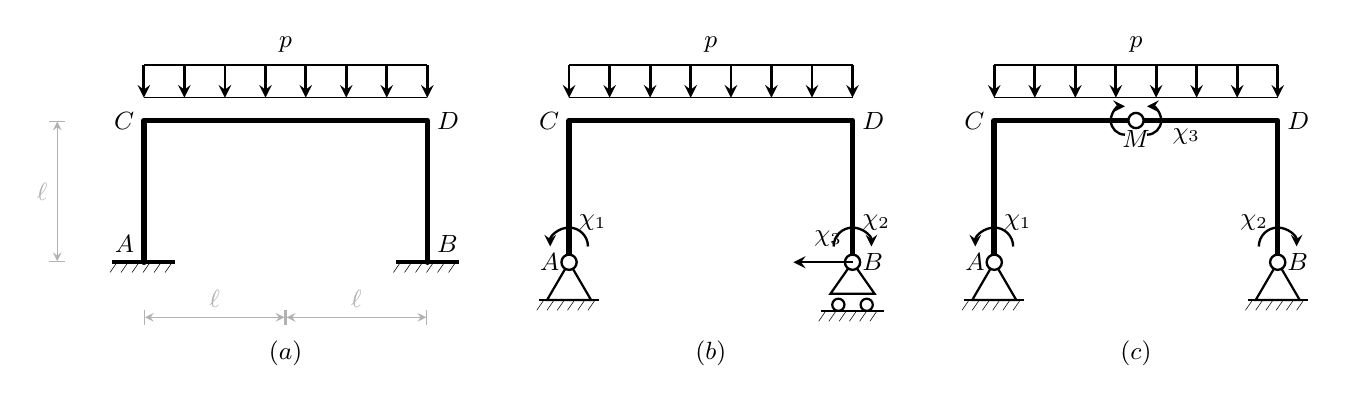
\begin{tikzpicture}[
					trave/.style={line width=2.0pt, line cap=round, line join=round, black},
					terra/.style={line width=0.8pt, black},
					carico/.style={->, >=stealth, line width=1.0pt, black},
					nodoV/.style={circle, fill=white, draw=black,
						inner sep=0pt, minimum size=5.5pt, line width=0.85pt},
					quota/.style={|<->|, >=stealth, thin, gray!60},
					]  
					
					\def\L{1.80}   % ℓ in cm
					\def\SEP{5.40} % separazione tra i pannelli
					\def\Lc{2.00}   % = \L + 0.20
					
					%%═══ PANNELLO (a) — portale doppiamente incastrato ══════════════════════
					\begin{scope}[xshift=0cm]
						%% Travi
						\draw[trave](0,0)--(0,\L)--(2*\L,\L)--(2*\L,0);
						%% Incastro in A
						\draw[terra,line width=1.4pt](-0.40,0)--(0.40,0);
						\foreach \x in {-0.34,-0.20,-0.06,0.08,0.22,0.36}
						\draw[very thin](\x,0)--++(-0.09,-0.13);
						%% Incastro in B
						\draw[terra,line width=1.4pt]({2*\L-0.40},0)--({2*\L+0.40},0);
						\foreach \x in {-0.34,-0.20,-0.06,0.08,0.22,0.36}
						\draw[very thin]({2*\L+\x},0)--++(-0.09,-0.13);
						%% Carico uniforme p
						\foreach \t in {0.0,0.143,0.286,0.429,0.571,0.714,0.857,1.00}{
							\draw[carico]({2*\L*\t},{\Lc+0.50})--({2*\L*\t},{\Lc+0.09});}
						\draw[black,line width=0.65pt](0,{\Lc+0.50})--(2*\L,{\Lc+0.50});
						\draw[black,line width=0.40pt](0,{\Lc+0.09})--(2*\L,{\Lc+0.09});
						\node[above,font=\small]at(\L,{\Lc+0.54}){$p$};
						%% Etichette nodi
						\node[above left,font=\small]at(0,0){$A$};
						\node[above right,font=\small]at(2*\L,0){$B$};
						\node[left,font=\small]at(0,\L){$C$};
						\node[right,font=\small]at(2*\L,\L){$D$};
						%% Quote dimensionali
						\draw[quota](-1.10,0)--(-1.10,\L)node[midway,left,font=\small]{$\ell$};
						\draw[quota](0,-0.70)--(\L,-0.70)node[midway,above,font=\small]{$\ell$};
						\draw[quota](\L,-0.70)--(2*\L,-0.70)node[midway,above,font=\small]{$\ell$};
						\node[font=\small]at(\L,-1.15){$(a)$};
					\end{scope}
					
					%%═══ PANNELLO (b) — sistema principale «portale appoggiato» ═════════════
					\begin{scope}[xshift=\SEP cm]
						%% Travi
						\draw[trave](0,0)--(0,\L)--(2*\L,\L)--(2*\L,0);
						%% Cerniera in A
						\draw[terra](0,0)--(-0.28,-0.48)--(0.28,-0.48)--cycle;
						\draw[terra](-0.38,-0.48)--(0.38,-0.48);
						\foreach \x in {-0.32,-0.19,-0.06,0.07,0.20,0.33}
						\draw[very thin](\x,-0.48)--++(-0.09,-0.13);
						\node[nodoV]at(0,0){};
						%% Carrello con piano di scorrimento orizzontale in B
						\draw[terra](2*\L,0)--(2*\L-0.28,-0.40)--(2*\L+0.28,-0.40)--cycle;
						\draw[terra](2*\L-0.18,-0.54)circle(2.2pt);
						\draw[terra](2*\L+0.18,-0.54)circle(2.2pt);
						\draw[terra]({2*\L-0.40},-0.62)--({2*\L+0.40},-0.62);
						\foreach \x in {-0.34,-0.21,-0.08,0.05,0.18,0.31}
						\draw[very thin]({2*\L+\x},-0.62)--++(-0.09,-0.13);
						\node[nodoV]at(2*\L,0){};
						%% Carico uniforme p
						\foreach \t in {0.0,0.143,0.286,0.429,0.571,0.714,0.857,1.00}{
							\draw[carico]({2*\L*\t},{\Lc+0.50})--({2*\L*\t},{\Lc+0.09});}
						\draw[black,line width=0.65pt](0,{\Lc+0.50})--(2*\L,{\Lc+0.50});
						\draw[black,line width=0.40pt](0,{\Lc+0.09})--(2*\L,{\Lc+0.09});
						\node[above,font=\small]at(\L,{\Lc+0.54}){$p$};
						%% Etichette nodi
						\node[left,font=\small]at(0,0){$A$};
						\node[right,font=\small]at(2*\L,0){$B$};
						\node[left,font=\small]at(0,\L){$C$};
						\node[right,font=\small]at(2*\L,\L){$D$};
						%% χ₁ — coppia antioraria in A: semiarco che attraversa la colonna,
						%%       convessità verso l'alto; centro (0, 0.20), raggio 0.24
						\draw[->,>=stealth,line width=0.85pt](0.24,0.20)arc(0:180:0.24);
						\node[right,font=\small]at(0,0.50){$\chi_1$};
						%% χ₂ — coppia oraria in B: semiarco speculare a χ₁,
						%%       centro (2ℓ, 0.20), raggio 0.24
						\draw[->,>=stealth,line width=0.85pt]({2*\L-0.24},0.20)arc(180:0:0.24);
						\node[right,font=\small]at(2*\L,0.50){$\chi_2$};
						%% χ₃ — reazione orizzontale rimossa: coda in B, punta verso A
						\draw[->,>=stealth,line width=0.90pt](2*\L,0)--({2*\L-0.75},0);
						\node[left=0.3,font=\small]at(2*\L,0.30){$\chi_3$};
						\node[font=\small]at(\L,-1.15){$(b)$};
					\end{scope}
					
					%%═══ PANNELLO (c) — sistema principale «portale a tre cerniere» ══════════
					\begin{scope}[xshift={2*\SEP cm}]
						%% Travi
						\draw[trave](0,0)--(0,\L)--(2*\L,\L)--(2*\L,0);
						%% Cerniera in A
						\draw[terra](0,0)--(-0.28,-0.48)--(0.28,-0.48)--cycle;
						\draw[terra](-0.38,-0.48)--(0.38,-0.48);
						\foreach \x in {-0.32,-0.19,-0.06,0.07,0.20,0.33}
						\draw[very thin](\x,-0.48)--++(-0.09,-0.13);
						\node[nodoV]at(0,0){};
						%% Cerniera in B
						\draw[terra](2*\L,0)--(2*\L-0.28,-0.48)--(2*\L+0.28,-0.48)--cycle;
						\draw[terra]({2*\L-0.38},-0.48)--({2*\L+0.38},-0.48);
						\foreach \x in {-0.32,-0.19,-0.06,0.07,0.20,0.33}
						\draw[very thin]({2*\L+\x},-0.48)--++(-0.09,-0.13);
						\node[nodoV]at(2*\L,0){};
						%% Cerniera interna in M (mezzeria del traverso)
						\node[nodoV]at(\L,\L){};
						%% Carico uniforme p
						\foreach \t in {0.0,0.143,0.286,0.429,0.571,0.714,0.857,1.00}{
							\draw[carico]({2*\L*\t},{\Lc+0.50})--({2*\L*\t},{\Lc+0.09});}
						\draw[black,line width=0.65pt](0,{\Lc+0.50})--(2*\L,{\Lc+0.50});
						\draw[black,line width=0.40pt](0,{\Lc+0.09})--(2*\L,{\Lc+0.09});
						\node[above,font=\small]at(\L,{\Lc+0.54}){$p$};
						%% Etichette nodi
						\node[left,font=\small]at(0,0){$A$};
						\node[right,font=\small]at(2*\L,0){$B$};
						\node[left,font=\small]at(0,\L){$C$};
						\node[right,font=\small]at(2*\L,\L){$D$};
						\node[below=0.04,font=\small]at(\L,\L){$M$};
						%% χ₁ — coppia antioraria in A (identica al pannello b)
						\draw[->,>=stealth,line width=0.85pt](0.24,0.20)arc(0:180:0.24);
						\node[right,font=\small]at(0,0.50){$\chi_1$};
						%% χ₂ — coppia oraria in B (identica al pannello b)
						\draw[->,>=stealth,line width=0.85pt]({2*\L-0.24},0.20)arc(180:0:0.24);
						\node[left,font=\small]at(2*\L,0.50){$\chi_2$};
						%% χ₃ — coppia interna in M: due semiarchi (stile trave continua)
						\draw[->,>=stealth,line width=0.85pt]({\L-0.14},{\L-0.18}) arc(270:90:0.18);
						\draw[->,>=stealth,line width=0.85pt]({\L+0.14},{\L-0.18}) arc(-90:90:0.18);
						\node[right=0.0,font=\small]at({\L+0.34},{\L-0.20}){$\chi_3$};
						\node[font=\small]at(\L,-1.15){$(c)$};
					\end{scope}
					
				\end{tikzpicture}
			}
			\caption{Portale doppiamente incastrato: schema iperstatico e due scelte
				del sistema principale.
				$(a)$~Schema originale, grado di iperstaticità $g_i = 3$
				($g_{\mathscr{i}}^{\text{est}} = 3$,
				$g_{\mathscr{i}}^{\text{int}} = 0$):
				colonne incastrate in $A$ e $B$, traverso $CD$ con carico
				uniforme~$p$.
				$(b)$~Sistema principale ``portale appoggiato'': gli incastri
				sono sostituiti da una cerniera in $A$ e da un carrello
				a reazione verticale in $B$; le incognite iperstatiche sono
				la coppia $\chi_1$ (momento rimosso in $A$, antioraria),
				la coppia $\chi_2$ (momento rimosso in $B$, oraria)
				e la forza orizzontale $\chi_3$ (reazione orizzontale rimossa
				in $B$, diretta verso $A$).
				$(c)$~Sistema principale ``portale a tre cerniere»'': gli incastri
				sono sostituiti da cerniere esterne in $A$ e $B$; una cerniera
				interna in $M$ (mezzeria del traverso) rilascia la continuità
				del momento flettente; le incognite iperstatiche sono la
				coppia $\chi_1$ in $A$, la coppia $\chi_2$ in $B$
				e la coppia $\chi_3$ in $M$.}
			\label{fig:portale_sistemi_principali}
		\end{figure}
		%%%%%%%%%%%%%%%%%%%%%%%%%%%%%%%%%%%%%%%%%%%
		
		
		
		
		\begin{oss}
			Il sistema principale~$(c)$ introduce una cerniera
			interna in~$M$, pur essendo l'iperstaticità del
			sistema originale interamente esterna.
			Questo non è una contraddizione: la scelta del sistema
			principale è libera, purché il sistema risultante
			sia isostatico e geometricamente stabile.
			La cerniera in~$M$ non rimuove una ridondanza interna
			del sistema originale --- che non ne ha --- ma
			costituisce semplicemente il modo più conveniente
			di eliminare la terza ridondanza esterna.
			L'incognita~$\chi_3$ rappresenta il valore del
			momento flettente nella sezione~$M$ del sistema
			originale, che la cerniera azzera nel sistema
			principale e che le autosoluzioni restituiscono.
		\end{oss}
		
		Si adotta il sistema principale~$(c)$.
		Esso è preferibile a~$(b)$ per due ragioni.
		Prima: la simmetria geometrica del portale e la simmetria
		del carico~$p$ implicano $\chi_1 = \chi_2$, riducendo
		i problemi indipendenti da tre a due.
		Seconda: il portale a tre cerniere è una struttura familiare
		e il suo comportamento sotto i carichi assegnati è
		immediatamente interpretabile.
		
		La soluzione del sistema originale si scrive per
		sovrapposizione~\eqref{eq:sol_iperstatica_telaio}:
		\begin{equation}\label{eq:portale_sovrapposizione}
			\begin{aligned}
				N &= N_0 + \chi_1\,N_1 + \chi_2\,N_2 + \chi_3\,N_3, \\
				T &= T_0 + \chi_1\,T_1 + \chi_2\,T_2 + \chi_3\,T_3, \\
				M &= M_0 + \chi_1\,M_1 + \chi_2\,M_2 + \chi_3\,M_3.
			\end{aligned}
		\end{equation}
		dove il pedice~$0$ denota la soluzione particolare
		(sistema principale sotto il carico~$p$, con
		$\chi_j = 0$) e i pedici~$1$,~$2$,~$3$ denotano le
		autosoluzioni (sistema principale sotto la sola
		incognita unitaria $\chi_j = 1$, senza carico esterno).
		
		
		%%%%%%%%%%%%%%%%%%%%%%%%%%%%%%%%%%%%%%%%%%%
		\begin{figure}[htbp]
			\centering
			\resizebox{\textwidth}{!}{%
				\begin{tikzpicture}[
					trave/.style={line width=1.8pt, line cap=round, line join=round, black},
					terra/.style={line width=0.8pt, black},
					nodoV/.style={circle, fill=white, draw=black,
						inner sep=0pt, minimum size=5pt, line width=0.80pt},
					reaz/.style={-{Stealth[length=5pt,width=4pt]}, line width=0.8pt, black},
					cop/.style={-{Stealth[length=4pt,width=3.5pt]}, line width=0.8pt, black},
					lab/.style={font=\small},
					etlab/.style={circle, draw=black, line width=0.6pt,
						fill=white, inner sep=1.5pt, font=\small},
					]
					
					\def\L{1.5}
					\def\AR{0.55}
					\def\HSEP{5.6}
					\def\VSEP{3.0}
					
					\def\portale{\draw[trave](0,0)--(0,\L)--(2*\L,\L)--(2*\L,0);}
					\def\cernieraA{%
						\draw[terra](0,0)--(-0.22,-0.36)--(0.22,-0.36)--cycle;
						\draw[terra](-0.30,-0.36)--(0.30,-0.36);
						\foreach \x in {-0.24,-0.12,0.00,0.12,0.24}
						\draw[very thin](\x,-0.36)--++(-0.08,-0.10);
						\node[nodoV]at(0,0){};}
					\def\cernieraB{%
						\draw[terra](2*\L,0)--(2*\L-0.22,-0.36)--(2*\L+0.22,-0.36)--cycle;
						\draw[terra]({2*\L-0.30},-0.36)--({2*\L+0.30},-0.36);
						\foreach \x in {-0.24,-0.12,0.00,0.12,0.24}
						\draw[very thin]({2*\L+\x},-0.36)--++(-0.08,-0.10);
						\node[nodoV]at(2*\L,0){};}
					\def\nodoM{\node[nodoV]at(\L,\L){};}
					\def\nodilabel{%
						\node[right,lab]at(0,0){$A$};
						\node[left,lab]at(2*\L,0){$B$};
						\node[below right,lab]at(0,\L){$C$};
						\node[below left,lab]at(2*\L,\L){$D$};
						\node[below,lab]at(\L,\L){$M$};}
					
					%% P0 -- riga 1 col 1
					\begin{scope}[xshift=0cm, yshift=0cm]
						%% carico distribuito p sul traverso
						\foreach \t in {0.0,0.143,0.286,0.429,0.571,0.714,0.857,1.00}
						\draw[reaz]({2*\L*\t},{\L+0.50})--({2*\L*\t},\L);
						\draw[black,line width=0.65pt](0,{\L+0.50})--(2*\L,{\L+0.50});
						\draw[black,line width=0.40pt](0,\L)--(2*\L,\L);
						\node[above,lab]at(\L,{\L+0.54}){$p$};
						%% reazioni in A
						\draw[reaz](0,{-\AR})--(0,0);
						\node[below,lab]at(0,{-\AR}){$p\ell$};
						\draw[reaz]({-\AR},0)--(0,0);
						\node[left,lab]at({-\AR},0){$\tfrac{p\ell}{2}$};
						%% reazioni in B
						\draw[reaz](2*\L,{-\AR})--(2*\L,0);
						\node[below,lab]at(2*\L,{-\AR}){$p\ell$};
						\draw[reaz]({2*\L+\AR},0)--(2*\L,0);
						\node[right,lab]at({2*\L+\AR},0){$\tfrac{p\ell}{2}$};
						\portale \cernieraA \cernieraB \nodoM \nodilabel
						\node[etlab]at(\L,{0}){$P0$};
					\end{scope}
					
					
					%% P1 -- riga 1 col 2
					\begin{scope}[xshift=\HSEP cm, yshift=0cm]
						%% coppia antioraria in A
						\draw[cop](0,0)+(-30:0.38) arc(-30:180:0.38);
						\node[above=0.2,lab]at({-0.28},0){$1$};
						%% VA su
						\draw[reaz](0,{-\AR})--(0,0);
						\node[below,lab]at(0,{-\AR}){$\tfrac{1}{2\ell}$};
						%% HA verso sinistra (esterno)
						\draw[reaz](0,0)--({-\AR},0);
						\node[left,lab]at({-\AR},0){$\tfrac{1}{2\ell}$};
						%% VB giu
						\draw[reaz](2*\L,0)--(2*\L,{-\AR});
						\node[below,lab]at(2*\L,{-\AR}){$\tfrac{1}{2\ell}$};
						%% HB verso destra (esterno)
						\draw[reaz](2*\L,0)--({2*\L+\AR},0);
						\node[right,lab]at({2*\L+\AR},0){$\tfrac{1}{2\ell}$};
						\portale \cernieraA \cernieraB \nodoM \nodilabel
						\node[etlab]at(\L,{0}){$P1$};
					\end{scope}
					
					%% P2 -- riga 2 col 1
					\begin{scope}[xshift=0cm, yshift={-\VSEP cm}]
						%% coppia oraria in B -- semicerchio 180 gradi, senso orario
						\draw[cop](2*\L-0.73,0.06)+(0:0.38) arc(180:-0:0.38);
						\node[above right,lab]at({2*\L+0.38},0){$1$};
						
						
						%			%% coppia oraria in B
						%			\draw[cop](2*\L,0)+(210:0.38) arc(210:510:0.38);
						%			\node[right=0.12,lab]at({2*\L+0.38},0){$1$};
						%% VA giu
						\draw[reaz](0,0)--(0,{-\AR});
						\node[below,lab]at(0,{-\AR}){$\tfrac{1}{2\ell}$};
						%% HA verso sinistra (esterno)
						\draw[reaz](0,0)--({-\AR},0);
						\node[left,lab]at({-\AR},0){$\tfrac{1}{2\ell}$};
						%% VB su
						\draw[reaz](2*\L,{-\AR})--(2*\L,0);
						\node[below,lab]at(2*\L,{-\AR}){$\tfrac{1}{2\ell}$};
						%% HB verso destra (esterno)
						\draw[reaz](2*\L,0)--({2*\L+\AR},0);
						\node[right,lab]at({2*\L+\AR},0){$\tfrac{1}{2\ell}$};
						\portale \cernieraA \cernieraB \nodoM \nodilabel
						\node[etlab]at(\L,{0}){$P2$};
					\end{scope}
					
					%% P3 -- riga 2 col 2
					\begin{scope}[xshift=\HSEP cm, yshift={-\VSEP cm}]
						%			%% coppia antioraria in M
						%			\draw[cop](\L,\L)+(-30:0.38) arc(-30:210:0.38);
						%			\node[above=0.44,lab]at(\L,\L){$1$};
						%% coppia antioraria a sinistra di M
						\draw[->,>=stealth,line width=0.85pt]({\L-0.14},{\L-0.18}) arc(270:90:0.18);
						%% coppia oraria a destra di M
						\draw[<-,>=stealth,line width=0.85pt]({\L+0.14},{\L+0.18}) arc(90:-90:0.18);
						\node[above,lab]at({\L},\L){$1$};
						%% HA verso destra (interno), HB verso sinistra (interno) -- VA=VB=0
						\draw[reaz]({-\AR},0)--(0,0);
						\node[left,lab]at({-\AR},0){$\tfrac{1}{\ell}$};
						\draw[reaz]({2*\L+\AR},0)--(2*\L,0);
						\node[right,lab]at({2*\L+\AR},0){$\tfrac{1}{\ell}$};
						\portale \cernieraA \cernieraB \nodoM \nodilabel
						\node[etlab]at(\L,{0}){$P3$};
					\end{scope}
					
				\end{tikzpicture}
			}
			\caption{Portale a tre cerniere: reazioni vincolari nei quattro problemi
				di carico. Pannello~$P0$: carico uniforme~$p$ sul traverso.
				Pannelli~$P1$, $P2$, $P3$: coppie unitarie $\chi_1$, $\chi_2$, $\chi_3$
				applicate rispettivamente in~$A$, $B$ e~$M$.}
			\label{fig:portale_reazioni:P0_1_2_3}
		\end{figure}
		
		Le reazioni vincolari del sistema principale nei quattro problemi
		di carico sono raccolte nella \FIGref{fig:portale_reazioni:P0_1_2_3}.
		
		
		\esottotit{Problema~0 --- sistema principale sotto il carico~$p$.}
		Seguendo la sequenza operativa del
		\CAPref{cap:sistemi_conn_eterogenee} --- equilibrio
		globale, isolamento dei semitravoni $CM$ e $MD$
		alla cerniera interna, equilibrio dei corpi liberi
		--- si ricavano le reazioni vincolari:
		\[
		V_A = V_B = p\ell \;\text{(verso l'alto)},
		\qquad
		H_A = H_B = \frac{p\ell}{2} \;\text{(verso l'interno)},
		\]
		dove la spinta orizzontale~$H$, diretta verso
		l'interno del portale in entrambi gli appoggi,
		è la caratteristica distintiva del portale a tre
		cerniere rispetto alla trave appoggiata.
		I diagrammi $N_0$,~$T_0$,~$M_0$ su ciascuna asta
		si ricavano per equilibrio dei corpi liberi e sono
		riportati nella \FIGref{fig:portale_problema0}.
		
		%%%%%%%%%%%%%%%%%%%%%%%%%%%%%%%%%%%%%%%%%%%
		\begin{figure}[htbp]
			\centering
			\resizebox{\textwidth}{!}{%
				\begin{tikzpicture}[
					trave/.style={line width=1.8pt, line cap=round, line join=round, black},
					terra/.style={line width=0.8pt, black},
					diag/.style={line width=0.90pt, black},
					nodoV/.style={circle, fill=white, draw=black,
						inner sep=0pt, minimum size=5.0pt, line width=0.80pt},
					segno/.style={circle, draw=black, fill=white, inner sep=0pt,
						minimum size=8pt, font=\tiny, line width=0.55pt},
					etlab/.style={circle, draw=black, line width=0.6pt,
						fill=white, inner sep=2pt, font=\small},
					lab/.style={font=\small},
					]
					
					\def\L{1.80}   % ℓ in cm
					\def\SEP{5.80} % separazione tra pannelli
					\def\dN{0.55}  % scala N: pℓ → 0.55 cm
					\def\dT{0.60}  % scala T: pℓ → 0.60 cm
					\def\dM{0.75}  % scala M: pℓ²/2 → 0.75 cm
					
					\def\portale{\draw[trave](0,0)--(0,\L)--(2*\L,\L)--(2*\L,0);}
					\def\cernieraA{%
						\draw[terra](0,0)--(-0.24,-0.40)--(0.24,-0.40)--cycle;
						\draw[terra](-0.34,-0.40)--(0.34,-0.40);
						\foreach \x in {-0.28,-0.16,-0.04,0.08,0.20,0.30}
						\draw[very thin](\x,-0.40)--++(-0.08,-0.11);
						\node[nodoV]at(0,0){};}
					\def\cernieraB{%
						\draw[terra](2*\L,0)--(2*\L-0.24,-0.40)--(2*\L+0.24,-0.40)--cycle;
						\draw[terra]({2*\L-0.34},-0.40)--({2*\L+0.34},-0.40);
						\foreach \x in {-0.28,-0.16,-0.04,0.08,0.20,0.30}
						\draw[very thin]({2*\L+\x},-0.40)--++(-0.08,-0.11);
						\node[nodoV]at(2*\L,0){};}
					
					%%═══ PANNELLO (a) — N₀ ══════════════════════════════════════════════
					\begin{scope}[xshift=0cm]
						%% N colonna sinistra (compressione, all'esterno = sinistra)
						\fill[gray!15](-\dN,0)--(0,0)--(0,\L)--(-\dN,\L)--cycle;
						\foreach \y in {0.15,0.30,...,1.75}
						{\draw[gray!50,very thin](-\dN,\y)--(0,\y);}
						\draw[diag](-\dN,0)--(-\dN,\L);
						\draw[diag](-\dN,0)--(0,0);
						\draw[diag](-\dN,\L)--(0,\L);
						%% N colonna destra (compressione, all'esterno = destra)
						\fill[gray!20](2*\L,0)--({2*\L+\dN},0)--({2*\L+\dN},\L)--(2*\L,\L)--cycle;
						\foreach \y in {0.15,0.30,...,1.75}
						{\draw[gray!50,very thin](2*\L,\y)--({2*\L+\dN},\y);}
						\draw[diag]({2*\L+\dN},0)--({2*\L+\dN},\L);
						\draw[diag](2*\L,0)--({2*\L+\dN},0);
						\draw[diag](2*\L,\L)--({2*\L+\dN},\L);
						%% N traverso (compressione, sotto — tratteggio verticale)
						\fill[gray!20](0,{\L-\dN/2})--(2*\L,{\L-\dN/2})--(2*\L,\L)--(0,\L)--cycle;
						\foreach \x in {0.35,0.70,...,3.50}
						{\draw[gray!50,very thin](\x,{\L-\dN/2})--(\x,\L);}
						\draw[diag](0,{\L-\dN/2})--(2*\L,{\L-\dN/2});
						%% Struttura
						\portale \cernieraA \cernieraB
						\node[nodoV]at(\L,\L){};
						%% Segni ±
						\node[segno]at({-\dN/2},{\L*0.50}){$-$};
						\node[segno]at({2*\L+\dN/2},{\L*0.50}){$-$};
						\node[segno]at({0.5*\L},{\L-\dN/4}){$-$};
						\node[segno]at({1.5*\L},{\L-\dN/4}){$-$};
						%% Valori
						\node[left=0.04,lab]at(-\dN,{\L*0.50}){$p\ell$};
						\node[right=0.04,lab]at({2*\L+\dN},{\L*0.50}){$p\ell$};
						\node[below=0.04,lab]at(\L,{\L-\dN/2}){$\tfrac{p\ell}{2}$};
						%% Etichette nodi
						\node[right,lab]at(0,0){$A$};
						\node[left,lab]at(2*\L,0){$B$};
						\node[above,lab]at(0,\L){$C$};
						\node[above,lab]at(2*\L,\L){$D$};
						\node[above,lab]at(\L,\L){$M$};
						%% Label cerchiata al centro del portale
						\node[etlab]at(\L,{0}){$N_0$};
					\end{scope}
					
					%%═══ PANNELLO (b) — T₀ ══════════════════════════════════════════════
					\begin{scope}[xshift=\SEP cm]
						%% T colonna sinistra (T = −pℓ/2, esterno = sinistra)
						\fill[gray!15]({-\dT/2},0)--(0,0)--(0,\L)--({-\dT/2},\L)--cycle;
						\foreach \y in {0.15,0.30,...,1.75}
						{\draw[gray!50,very thin]({-\dT/2},\y)--(0,\y);}
						\draw[diag]({-\dT/2},0)--({-\dT/2},\L);
						\draw[diag]({-\dT/2},0)--(0,0);
						\draw[diag]({-\dT/2},\L)--(0,\L);
						%% T colonna destra (T = +pℓ/2, esterno = destra)
						\fill[gray!15](2*\L,0)--({2*\L+\dT/2},0)--({2*\L+\dT/2},\L)--(2*\L,\L)--cycle;
						\foreach \y in {0.15,0.30,...,1.75}
						{\draw[gray!50,very thin](2*\L,\y)--({2*\L+\dT/2},\y);}
						\draw[diag]({2*\L+\dT/2},0)--({2*\L+\dT/2},\L);
						\draw[diag](2*\L,0)--({2*\L+\dT/2},0);
						\draw[diag](2*\L,\L)--({2*\L+\dT/2},\L);
						%% T traverso parte positiva (C→M, sopra — tratteggio verticale)
						\fill[gray!15](0,\L)--(0,{\L+\dT})--(\L,\L)--cycle;
						\begin{scope}
							\clip(0,\L)--(0,{\L+\dT})--(\L,\L)--cycle;
							\foreach \x in {0.25,0.50,...,1.75}
							{\draw[gray!50,very thin](\x,{\L-0.1})--(\x,{\L+\dT+0.1});}
						\end{scope}
						\draw[diag](0,{\L+\dT})--(\L,\L);
						\draw[diag](0,\L)--(0,{\L+\dT});
						%% T traverso parte negativa (M→D, sotto — tratteggio verticale)
						\fill[gray!15](\L,\L)--(2*\L,{\L-\dT})--(2*\L,\L)--cycle;
						\begin{scope}
							\clip(\L,\L)--(2*\L,{\L-\dT})--(2*\L,\L)--cycle;
							\foreach \x in {1.95,2.20,...,3.55}
							{\draw[gray!50,very thin](\x,{\L-\dT-0.1})--(\x,{\L+0.1});}
						\end{scope}
						\draw[diag](\L,\L)--(2*\L,{\L-\dT});
						\draw[diag](2*\L,{\L-\dT})--(2*\L,\L);
						%% Struttura
						\portale \cernieraA \cernieraB
						\node[nodoV]at(\L,\L){};
						%% Segni ±
						\node[segno]at({-\dT/4},{\L*0.50}){$-$};
						\node[segno]at({2*\L+\dT/4},{\L*0.50}){$+$};
						\node[segno]at({0.28*\L},{\L+0.22}){$+$};
						\node[segno]at({1.72*\L},{\L-0.22}){$-$};
						%% Valori
						\node[left=0.04,lab]at({-\dT/2},{\L*0.50}){$\tfrac{p\ell}{2}$};
						\node[right=0.04,lab]at({2*\L+\dT/2},{\L*0.50}){$\tfrac{p\ell}{2}$};
						\node[left=0.04,lab]at(0,{\L+\dT}){$p\ell$};
						\node[right=0.04,lab]at({2*\L-0.60},{\L-\dT-0.2}){$p\ell$};
						%% Etichette nodi
						\node[right,lab]at(0,0){$A$};
						\node[left,lab]at(2*\L,0){$B$};
						\node[above left,lab]at(0,\L){$C$};
						\node[above,lab]at(2*\L,\L){$D$};
						\node[above,lab]at(\L,\L){$M$};
						%% Label cerchiata al centro del portale
						\node[etlab]at(\L,{0}){$T_0$};
					\end{scope}
					
					%%═══ PANNELLO (c) — M₀ ══════════════════════════════════════════════
					\begin{scope}[xshift={2*\SEP cm}]
						%% M colonna sinistra (lineare 0→−pℓ²/2, a sinistra — tratteggio orizzontale)
						\fill[gray!15](0,0)--(-\dM,\L)--(0,\L)--cycle;
						\begin{scope}
							\clip(0,0)--(-\dM,\L)--(0,\L)--cycle;
							\foreach \y in {0.15,0.30,...,1.75}
							{\draw[gray!50,very thin]({-\dM-0.1},\y)--(0.1,\y);}
						\end{scope}
						\draw[diag](0,0)--(-\dM,\L);
						\draw[diag](-\dM,\L)--(0,\L);
						%% M colonna destra (lineare 0→−pℓ²/2, a destra — tratteggio orizzontale)
						\fill[gray!15](2*\L,0)--({2*\L+\dM},\L)--(2*\L,\L)--cycle;
						\begin{scope}
							\clip(2*\L,0)--({2*\L+\dM},\L)--(2*\L,\L)--cycle;
							\foreach \y in {0.15,0.30,...,1.75}
							{\draw[gray!50,very thin](2*\L-0.1,\y)--({2*\L+\dM+0.1},\y);}
						\end{scope}
						\draw[diag](2*\L,0)--({2*\L+\dM},\L);
						\draw[diag]({2*\L+\dM},\L)--(2*\L,\L);
						%% M traverso (parabolico sopra — tratteggio verticale)
						\fill[gray!15](0,\L)--(0,{\L+\dM})
						-- plot[domain=0:2*\L,samples=40]({\x},{\L+\dM*((\x-\L)/\L)^2})
						-- (2*\L,\L)--cycle;
						\begin{scope}
							\clip(0,\L)--(0,{\L+\dM})
							-- plot[domain=0:2*\L,samples=40]({\x},{\L+\dM*((\x-\L)/\L)^2})
							-- (2*\L,\L)--cycle;
							\foreach \x in {0.25,0.50,...,3.55}
							{\draw[gray!50,very thin](\x,{\L-0.1})--(\x,{\L+\dM+0.1});}
						\end{scope}
						\draw[diag] plot[domain=0:2*\L,samples=40]
						({\x},{\L+\dM*((\x-\L)/\L)^2});
						\draw[diag](0,\L)--(0,{\L+\dM});
						\draw[diag](2*\L,\L)--(2*\L,{\L+\dM});
						%% Archetti di continuità in C e D (quarto di cerchio, raggio \dM)
						\draw[diag](-\dM,\L) arc(180:90:\dM);      % C: sinistra → alto
						\draw[diag](2*\L,{\L+\dM}) arc(90:0:\dM);  % D: alto → destra
						%% Struttura
						\portale \cernieraA \cernieraB
						\node[nodoV]at(\L,\L){};
						%% Valori
						\node[left=0.04,lab]at(-\dM,\L){$\tfrac{p\ell^2}{2}$};
						\node[right=0.04,lab]at({2*\L+\dM},\L){$\tfrac{p\ell^2}{2}$};
						%% Etichette nodi
						\node[below left,lab]at(0,0){$A$};
						\node[below right,lab]at(2*\L,0){$B$};
						\node[left,lab]at(0,{\L+0.20}){$C$};
						\node[right,lab]at(2*\L,{\L+0.20}){$D$};
						\node[below=0.04,lab]at(\L,\L){$M$};
						%% Label cerchiata al centro del portale
						\node[etlab]at(\L,{0}){$M_0$};
					\end{scope}
					
				\end{tikzpicture}
			}%
			\caption{Problema~$0$: diagrammi di $N_0$, $T_0$ e $M_0$
				sul portale a tre cerniere sotto il carico uniforme~$p$.
				Gli archetti in $C$ e $D$ indicano la continuità del momento
				flettente ai nodi rigidi.}
			\label{fig:portale_problema0}
		\end{figure}
		%%%%%%%%%%%%%%%%%%%%%%%%%%%%%%%%%%%%%%%%%%%
		
		
		
		\esottotit{Problema~1 --- autosoluzione $\chi_1 = 1$.}
		Il sistema principale è soggetto alla sola coppia
		unitaria $\chi_1 = 1$ applicata in~$A$, senza carichi
		esterni. Applicando la sequenza operativa del
		\CAPref{cap:sistemi_conn_eterogenee} si ricavano
		le reazioni vincolari:
		\[
		V_A = -V_B = \frac{1}{2\ell},
		\qquad
		H_A = H_B = \frac{1}{2\ell} \;\text{(verso l'esterno del portale)}.
		\]
		Le tre equazioni di equilibrio globale, integrate
		dalla condizione di momento nullo in~$M$ scritta
		per uno dei due semicerchi, forniscono le quattro
		equazioni necessarie a determinare le quattro
		incognite reattive.
		I diagrammi $N_1$,~$T_1$,~$M_1$ sono riportati
		nella \FIGref{fig:portale_autosoluzione_1}.
		
		
		%%%%%%%%%%%%%%%%%%%%%%%%%%%%%%%%%%%%%%%%%%%
		\begin{figure}[htbp]
			\centering
			\resizebox{\textwidth}{!}{%
				\begin{tikzpicture}[
					trave/.style={line width=1.8pt, line cap=round, line join=round, black},
					terra/.style={line width=0.8pt, black},
					diag/.style={line width=0.90pt, black},
					nodoV/.style={circle, fill=white, draw=black,
						inner sep=0pt, minimum size=5.0pt, line width=0.80pt},
					segno/.style={circle, draw=black, fill=white, inner sep=0pt,
						minimum size=8pt, font=\tiny, line width=0.55pt},
					etlab/.style={circle, draw=black, line width=0.6pt,
						fill=white, inner sep=2pt, font=\small},
					lab/.style={font=\small},
					]
					
					\def\L{1.80}
					\def\SEP{5.80}
					\def\dNo{0.55}
					\def\dTo{0.30}
					\def\dMo{0.75}
					\def\ext{0.09}  % estensione sopra traverso per visibilità chiusura in D
					
					\def\portale{\draw[trave](0,0)--(0,\L)--(2*\L,\L)--(2*\L,0);}
					\def\cernieraA{%
						\draw[terra](0,0)--(-0.24,-0.40)--(0.24,-0.40)--cycle;
						\draw[terra](-0.34,-0.40)--(0.34,-0.40);
						\foreach \x in {-0.28,-0.16,-0.04,0.08,0.20,0.30}
						\draw[very thin](\x,-0.40)--++(-0.08,-0.11);
						\node[nodoV]at(0,0){};}
					\def\cernieraB{%
						\draw[terra](2*\L,0)--(2*\L-0.24,-0.40)--(2*\L+0.24,-0.40)--cycle;
						\draw[terra]({2*\L-0.34},-0.40)--({2*\L+0.34},-0.40);
						\foreach \x in {-0.28,-0.16,-0.04,0.08,0.20,0.30}
						\draw[very thin]({2*\L+\x},-0.40)--++(-0.08,-0.11);
						\node[nodoV]at(2*\L,0){};}
					
					%%═══ PANNELLO (a) — N₁ ═════════════════════════════════════════════════
					\begin{scope}[xshift=0cm]
						\fill[gray!20](-\dNo,0)--(0,0)--(0,\L)--(-\dNo,\L)--cycle;
						\foreach \y in {0.15,0.30,...,1.75}{\draw[gray!50,very thin](-\dNo,\y)--(0,\y);}
						\draw[diag](-\dNo,0)--(-\dNo,\L);
						\draw[diag](-\dNo,0)--(0,0);
						\draw[diag](-\dNo,\L)--(0,\L);
						\fill[gray!20]({2*\L-\dNo},0)--(2*\L,0)--(2*\L,\L)--({2*\L-\dNo},\L)--cycle;
						\foreach \y in {0.15,0.30,...,1.75}{\draw[gray!50,very thin]({2*\L-\dNo},\y)--(2*\L,\y);}
						\draw[diag]({2*\L-\dNo},0)--({2*\L-\dNo},\L);
						\draw[diag]({2*\L-\dNo},0)--(2*\L,0);
						\draw[diag]({2*\L-\dNo},\L)--(2*\L,\L);
						\fill[gray!20](0,\L)--(2*\L,\L)--(2*\L,{\L+\dNo})--(0,{\L+\dNo})--cycle;
						\foreach \x in {0.35,0.70,...,3.50}{\draw[gray!50,very thin](\x,\L)--(\x,{\L+\dNo});}
						\draw[diag](0,{\L+\dNo})--(2*\L,{\L+\dNo});
						\draw[diag](0,\L)--(0,{\L+\dNo});
						\draw[diag](2*\L,\L)--(2*\L,{\L+\dNo});
						\portale \cernieraA \cernieraB
						\node[nodoV]at(\L,\L){};
						\node[segno]at({-\dNo/2},{\L*0.50}){$-$};
						\node[segno]at({2*\L-\dNo/2},{\L*0.50}){$+$};
						\node[segno]at({0.5*\L},{\L+\dNo/2}){$+$};
						\node[segno]at({1.5*\L},{\L+\dNo/2}){$+$};
						\node[left=0.04,lab]at(-\dNo,{\L*0.50}){$\tfrac{1}{2\ell}$};
						\node[left=0.04,lab]at({2*\L-\dNo},{\L*0.50}){$\tfrac{1}{2\ell}$};
						\node[above=0.04,lab]at(\L,{\L+\dNo}){$\tfrac{1}{2\ell}$};
						\node[right,lab]at(0,0){$A$};
						\node[right,lab]at(2*\L,0){$B$};
						\node[above left,lab]at(0,\L){$C$};
						\node[above right,lab]at(2*\L,\L){$D$};
						\node[below,lab]at(\L,\L){$M$};
						\node[etlab]at(\L,{0}){$N_1$};
					\end{scope}
					
					%%═══ PANNELLO (b) — T₁ ═════════════════════════════════════════════════
					\begin{scope}[xshift=\SEP cm]
						\fill[gray!20](0,0)--(\dTo,0)--(\dTo,\L)--(0,\L)--cycle;
						\foreach \y in {0.15,0.30,...,1.75}{\draw[gray!50,very thin](0,\y)--(\dTo,\y);}
						\draw[diag](\dTo,0)--(\dTo,\L);
						\draw[diag](0,0)--(\dTo,0);
						\draw[diag](0,\L)--(\dTo,\L);
						\fill[gray!20]({2*\L-\dTo},0)--(2*\L,0)--(2*\L,\L)--({2*\L-\dTo},\L)--cycle;
						\foreach \y in {0.15,0.30,...,1.75}{\draw[gray!50,very thin]({2*\L-\dTo},\y)--(2*\L,\y);}
						\draw[diag]({2*\L-\dTo},0)--({2*\L-\dTo},\L);
						\draw[diag]({2*\L-\dTo},0)--(2*\L,0);
						\draw[diag]({2*\L-\dTo},\L)--(2*\L,\L);
						\fill[gray!20](0,\L)--(2*\L,\L)--(2*\L,{\L+\dTo})--(0,{\L+\dTo})--cycle;
						\foreach \x in {0.35,0.70,...,3.50}{\draw[gray!50,very thin](\x,\L)--(\x,{\L+\dTo});}
						\draw[diag](0,{\L+\dTo})--(2*\L,{\L+\dTo});
						\draw[diag](0,\L)--(0,{\L+\dTo});
						\draw[diag](2*\L,\L)--(2*\L,{\L+\dTo});
						\portale \cernieraA \cernieraB
						\node[nodoV]at(\L,\L){};
						\node[segno]at(\dTo/2,{\L*0.50}){$+$};
						\node[segno]at({2*\L-\dTo/2},{\L*0.50}){$-$};
						\node[segno]at({0.5*\L},{\L+\dTo/2}){$+$};
						\node[segno]at({1.5*\L},{\L+\dTo/2}){$+$};
						\node[right=0.04,lab]at(\dTo,{\L*0.50}){$\tfrac{1}{2\ell}$};
						\node[left=0.04,lab]at({2*\L-\dTo},{\L*0.50}){$\tfrac{1}{2\ell}$};
						\node[above=0.04,lab]at(\L,{\L+\dTo}){$\tfrac{1}{2\ell}$};
						\node[left,lab]at(0,0){$A$};
						\node[right,lab]at(2*\L,0){$B$};
						\node[above left,lab]at(0,\L){$C$};
						\node[above right,lab]at(2*\L,\L){$D$};
						\node[below,lab]at(\L,\L){$M$};
						\node[etlab]at(\L,{0}){$T_1$};
					\end{scope}
					
					%%═══ PANNELLO (c) — M₁ ═════════════════════════════════════════════════
					\begin{scope}[xshift={2*\SEP cm}]
						%% M col. sin. (negativo, trapezio a sinistra: dMo in A, dMo/2 in C)
						\fill[gray!20](0,0)--(-\dMo,0)--(-\dMo/2,\L)--(0,\L)--cycle;
						\begin{scope}
							\clip(0,0)--(-\dMo,0)--(-\dMo/2,\L)--(0,\L)--cycle;
							\foreach \y in {0.15,0.30,...,1.75}
							{\draw[gray!50,very thin]({-\dMo-0.1},\y)--(0.1,\y);}
						\end{scope}
						\draw[diag](-\dMo,0)--(-\dMo/2,\L);
						\draw[diag](-\dMo,0)--(0,0);
						\draw[diag](-\dMo/2,\L)--(0,\L);
						%% M col. des. (positivo, triangolo a sinistra di BD — fibra tesa interna)
						\fill[gray!20](2*\L,0)--(2*\L,\L)--({2*\L-\dMo/2},\L)--cycle;
						\begin{scope}
							\clip(2*\L,0)--(2*\L,\L)--({2*\L-\dMo/2},\L)--cycle;
							\foreach \y in {0.15,0.30,...,1.75}
							{\draw[gray!50,very thin]({2*\L-\dMo/2-0.1},\y)--(2*\L+0.1,\y);}
						\end{scope}
						\draw[diag](2*\L,0)--({2*\L-\dMo/2},\L);   % faccia inclinata
						\draw[diag]({2*\L-\dMo/2},\L)--(2*\L,\L);   % chiusura in D (coperta dalla trave)
						%% M traverso metà sin. (negativo, triangolo sopra: dMo/2 in C, 0 in M)
						\fill[gray!20](0,\L)--(0,{\L+\dMo/2})--(\L,\L)--cycle;
						\begin{scope}
							\clip(0,\L)--(0,{\L+\dMo/2})--(\L,\L)--cycle;
							\foreach \x in {0.25,0.50,...,1.75}
							{\draw[gray!50,very thin](\x,{\L-0.1})--(\x,{\L+\dMo/2+0.1});}
						\end{scope}
						\draw[diag](0,{\L+\dMo/2})--(\L,\L);
						\draw[diag](0,\L)--(0,{\L+\dMo/2});
						%% M traverso metà des. (positivo, triangolo sotto: 0 in M, dMo/2 in D)
						\fill[gray!20](\L,\L)--(2*\L,{\L-\dMo/2})--(2*\L,\L)--cycle;
						\begin{scope}
							\clip(\L,\L)--(2*\L,{\L-\dMo/2})--(2*\L,\L)--cycle;
							\foreach \x in {1.90,2.15,...,3.55}
							{\draw[gray!50,very thin](\x,{\L-\dMo/2-0.1})--(\x,{\L+0.1});}
						\end{scope}
						\draw[diag](\L,\L)--(2*\L,{\L-\dMo/2});
						\draw[diag](2*\L,{\L-\dMo/2})--(2*\L,\L);
						%% Archetto di continuità in C (col. sin. → trav. sin.)
						\draw[diag](-\dMo/2,\L) arc(180:90:\dMo/2);
						%% Archetto di continuità in D (trav. des. → col. des.)
						\draw[diag](2*\L,{\L-\dMo/2}) arc(270:180:\dMo/2);
						%% Struttura
						\portale \cernieraA \cernieraB
						\node[nodoV]at(\L,\L){};
						%% Valori
						\node[left=0.04,lab]at(-\dMo,0){$1$};
						\node[above left=0.02,lab]at(-\dMo/2,\L){$\tfrac{1}{2}$};
						\node[above,lab]at({2*\L-\dMo/4},{\L+\ext}){$\tfrac{1}{2}$};
						\node[right=0.04,lab]at(2*\L,{\L-\dMo/2}){$\tfrac{1}{2}$};
						%% Etichette nodi
						\node[right,lab]at(0,0){$A$};
						\node[right,lab]at(2*\L,0){$B$};
						\node[below right,lab]at(0,\L){$C$};
						\node[right,lab]at(2*\L,\L){$D$};
						\node[below=0.04,lab]at(\L,\L){$M$};
						\node[etlab]at(\L,{0}){$M_1$};
					\end{scope}
					
				\end{tikzpicture}
			}%
			\caption{Autosoluzione~$1$ ($\chi_1 = 1$, coppia unitaria in~$A$):
				diagrammi di $N_1$, $T_1$ e $M_1$ sul portale a tre cerniere.
				L'archetto in~$C$ indica la continuità del momento flettente
				al nodo rigido.}
			\label{fig:portale_autosoluzione1}
		\end{figure}
		%%%%%%%%%%%%%%%%%%%%%%%%%%%%%%%%%%%%%%%%%%%
		
		\esottotit{Problema~2 --- autosoluzione $\chi_2 = 1$.}
		Per la simmetria geometrica del portale, i diagrammi
		$(N_2,\,T_2,\,M_2)$, riportati nella
		\FIGref{fig:portale_autosoluzione2}, si ricavano da
		$(N_1,\,T_1,\,M_1)$: le forme sono il riflesso speculare
		di quelle del Problema~$1$, con il segno di $N_2$ e $T_2$
		invertito rispetto a $N_1$ e $T_1$, mentre $M_2$ è il
		riflesso di $M_1$ con segno invariato.
		
		
		%%%%%%%%%%%%%%%%%%%%%%%%%%%%%%%%%%%%%%%%%%%
		\begin{figure}[htbp]
			\centering
			\resizebox{\textwidth}{!}{%
				\begin{tikzpicture}[
					trave/.style={line width=1.8pt, line cap=round, line join=round, black},
					terra/.style={line width=0.8pt, black},
					diag/.style={line width=0.90pt, black},
					nodoV/.style={circle, fill=white, draw=black,
						inner sep=0pt, minimum size=5.0pt, line width=0.80pt},
					segno/.style={circle, draw=black, fill=white, inner sep=0pt,
						minimum size=8pt, font=\tiny, line width=0.55pt},
					etlab/.style={circle, draw=black, line width=0.6pt,
						fill=white, inner sep=2pt, font=\small},
					lab/.style={font=\small},
					]
					
					\def\L{1.80}
					\def\SEP{5.80}
					\def\dNo{0.55}
					\def\dTo{0.30}
					\def\dMo{0.75}
					
					\def\portale{\draw[trave](0,0)--(0,\L)--(2*\L,\L)--(2*\L,0);}
					\def\cernieraA{%
						\draw[terra](0,0)--(-0.24,-0.40)--(0.24,-0.40)--cycle;
						\draw[terra](-0.34,-0.40)--(0.34,-0.40);
						\foreach \x in {-0.28,-0.16,-0.04,0.08,0.20,0.30}
						\draw[very thin](\x,-0.40)--++(-0.08,-0.11);
						\node[nodoV]at(0,0){};}
					\def\cernieraB{%
						\draw[terra](2*\L,0)--(2*\L-0.24,-0.40)--(2*\L+0.24,-0.40)--cycle;
						\draw[terra]({2*\L-0.34},-0.40)--({2*\L+0.34},-0.40);
						\foreach \x in {-0.28,-0.16,-0.04,0.08,0.20,0.30}
						\draw[very thin]({2*\L+\x},-0.40)--++(-0.08,-0.11);
						\node[nodoV]at(2*\L,0){};}
					
					%%═══ PANNELLO (a) — N₂ ═════════════════════════════════════════════════
					%% Specchio di N₁: col.sin=trazione(+) interno, col.des=compressione(-) esterno
					%%                 traverso=compressione(-) sotto
					\begin{scope}[xshift=0cm]
						%% Col. sin.: trazione (+), interno (destra di AC)
						\fill[gray!15](0,0)--(\dNo,0)--(\dNo,\L)--(0,\L)--cycle;
						\foreach \y in {0.15,0.30,...,1.75}{\draw[gray!50,very thin](0,\y)--(\dNo,\y);}
						\draw[diag](\dNo,0)--(\dNo,\L);
						\draw[diag](0,0)--(\dNo,0);
						\draw[diag](0,\L)--(\dNo,\L);
						%% Col. des.: compressione (-), esterno (destra di BD)
						\fill[gray!15](2*\L,0)--({2*\L+\dNo},0)--({2*\L+\dNo},\L)--(2*\L,\L)--cycle;
						\foreach \y in {0.15,0.30,...,1.75}{\draw[gray!50,very thin](2*\L,\y)--({2*\L+\dNo},\y);}
						\draw[diag]({2*\L+\dNo},0)--({2*\L+\dNo},\L);
						\draw[diag](2*\L,0)--({2*\L+\dNo},0);
						\draw[diag](2*\L,\L)--({2*\L+\dNo},\L);
						%% Traverso: compressione (-), sopra (evita sovrapposizione con col.sin)
						\fill[gray!15](0,\L)--(2*\L,\L)--(2*\L,{\L+\dNo})--(0,{\L+\dNo})--cycle;
						\foreach \x in {0.35,0.70,...,3.50}{\draw[gray!50,very thin](\x,\L)--(\x,{\L+\dNo});}
						\draw[diag](0,{\L+\dNo})--(2*\L,{\L+\dNo});
						\draw[diag](0,\L)--(0,{\L+\dNo});
						\draw[diag](2*\L,\L)--(2*\L,{\L+\dNo});
						\portale \cernieraA \cernieraB
						%% Trattini mancanti: bordo sup. del rettangolo di col.sin (coperto dalla trave)
						%% Ridisegnati 0.06 cm sopra il centro-trave, dove sono visibili sul fondo grigio
						\draw[diag](\dNo,\L)--(\dNo,{\L+0.06});       % prolungamento bordo destro
						\node[nodoV]at(\L,\L){};
						\node[segno]at(\dNo/2,{\L*0.50}){$+$};
						\node[segno]at({2*\L+\dNo/2},{\L*0.50}){$-$};
						\node[segno]at({0.5*\L},{\L+\dNo/2}){$-$};
						\node[segno]at({1.5*\L},{\L+\dNo/2}){$-$};
						\node[right=0.04,lab]at(\dNo,{\L*0.50}){$\tfrac{1}{2\ell}$};
						\node[right=0.04,lab]at({2*\L+\dNo},{\L*0.50}){$\tfrac{1}{2\ell}$};
						\node[above=0.04,lab]at(\L,{\L+\dNo}){$\tfrac{1}{2\ell}$};
						\node[left,lab]at(0,0){$A$};
						\node[left,lab]at(2*\L,0){$B$};
						\node[above left,lab]at(0,\L){$C$};
						\node[above right,lab]at(2*\L,\L){$D$};
						\node[above,lab]at(\L,\L){$M$};
						\node[etlab]at(\L,{0}){$N_2$};
					\end{scope}
					
					%%═══ PANNELLO (b) — T₂ ═════════════════════════════════════════════════
					%% Specchio di T₁: col.sin=(-) esterno, col.des=(+) esterno, traverso=(-) sotto
					\begin{scope}[xshift=\SEP cm]
						%% Col. sin.: (-), esterno (sinistra di AC)
						\fill[gray!15]({-\dTo},0)--(0,0)--(0,\L)--({-\dTo},\L)--cycle;
						\foreach \y in {0.15,0.30,...,1.75}{\draw[gray!50,very thin]({-\dTo},\y)--(0,\y);}
						\draw[diag]({-\dTo},0)--({-\dTo},\L);
						\draw[diag]({-\dTo},0)--(0,0);
						\draw[diag]({-\dTo},\L)--(0,\L);
						%% Col. des.: (+), esterno (destra di BD)
						\fill[gray!15](2*\L,0)--({2*\L+\dTo},0)--({2*\L+\dTo},\L)--(2*\L,\L)--cycle;
						\foreach \y in {0.15,0.30,...,1.75}{\draw[gray!50,very thin](2*\L,\y)--({2*\L+\dTo},\y);}
						\draw[diag]({2*\L+\dTo},0)--({2*\L+\dTo},\L);
						\draw[diag](2*\L,0)--({2*\L+\dTo},0);
						\draw[diag](2*\L,\L)--({2*\L+\dTo},\L);
						%% Traverso: (-), sotto
						\fill[gray!15](0,{\L-\dTo})--(2*\L,{\L-\dTo})--(2*\L,\L)--(0,\L)--cycle;
						\foreach \x in {0.35,0.70,...,3.50}{\draw[gray!50,very thin](\x,{\L-\dTo})--(\x,\L);}
						\draw[diag](0,{\L-\dTo})--(2*\L,{\L-\dTo});
						\portale \cernieraA \cernieraB
						\node[nodoV]at(\L,\L){};
						\node[segno]at({-\dTo/2},{\L*0.50}){$-$};
						\node[segno]at({2*\L+\dTo/2},{\L*0.50}){$+$};
						\node[segno]at({0.5*\L},{\L-\dTo/2}){$-$};
						\node[segno]at({1.5*\L},{\L-\dTo/2}){$-$};
						\node[left=0.04,lab]at({-\dTo},{\L*0.50}){$\tfrac{1}{2\ell}$};
						\node[right=0.04,lab]at({2*\L+\dTo},{\L*0.50}){$\tfrac{1}{2\ell}$};
						\node[below=0.04,lab]at(\L,{\L-\dTo}){$\tfrac{1}{2\ell}$};
						\node[right,lab]at(0,0){$A$};
						\node[left,lab]at(2*\L,0){$B$};
						\node[above,lab]at(0,\L){$C$};
						\node[above,lab]at(2*\L,\L){$D$};
						\node[above,lab]at(\L,\L){$M$};
						\node[etlab]at(\L,{0}){$T_2$};
					\end{scope}
					
					%%═══ PANNELLO (c) — M₂ ═════════════════════════════════════════════════
					%% Specchio di M₁:
					%%   col.sin = triangolo interno destra (0 in A, 1/2 in C)  ← specchio col.des di M₁
					%%   col.des = trapezio esterno destra (1 in B, 1/2 in D)   ← specchio col.sin di M₁
					%%   trav.sin = triangolo sotto (1/2 in C, 0 in M)          ← specchio trav.des di M₁
					%%   trav.des = triangolo sopra (0 in M, 1/2 in D)          ← specchio trav.sin di M₁
					\begin{scope}[xshift={2*\SEP cm}]
						%% M col. sin. (positivo, triangolo a destra di AC — fibra tesa interna)
						\fill[gray!15](0,0)--(0,\L)--(\dMo/2,\L)--cycle;
						\begin{scope}
							\clip(0,0)--(0,\L)--(\dMo/2,\L)--cycle;
							\foreach \y in {0.15,0.30,...,1.75}
							{\draw[gray!50,very thin]({-0.1},\y)--(\dMo/2+0.1,\y);}
						\end{scope}
						\draw[diag](0,0)--(\dMo/2,\L);         % faccia inclinata
						\draw[diag](\dMo/2,\L)--(0,\L);         % chiusura in C (coperta dalla trave)
						%% M col. des. (negativo, trapezio a destra di BD — fibra tesa esterna)
						\fill[gray!15](2*\L,0)--({2*\L+\dMo},0)--({2*\L+\dMo/2},\L)--(2*\L,\L)--cycle;
						\begin{scope}
							\clip(2*\L,0)--({2*\L+\dMo},0)--({2*\L+\dMo/2},\L)--(2*\L,\L)--cycle;
							\foreach \y in {0.15,0.30,...,1.75}
							{\draw[gray!50,very thin](2*\L-0.1,\y)--({2*\L+\dMo+0.1},\y);}
						\end{scope}
						\draw[diag]({2*\L+\dMo},0)--({2*\L+\dMo/2},\L);   % faccia inclinata
						\draw[diag](2*\L,0)--({2*\L+\dMo},0);              % base
						\draw[diag]({2*\L+\dMo/2},\L)--(2*\L,\L);          % chiusura in D (coperta)
						%% M traverso metà sin. (positivo, triangolo sotto: 1/2 in C, 0 in M)
						\fill[gray!15](0,\L)--(0,{\L-\dMo/2})--(\L,\L)--cycle;
						\begin{scope}
							\clip(0,\L)--(0,{\L-\dMo/2})--(\L,\L)--cycle;
							\foreach \x in {0.25,0.50,...,1.75}
							{\draw[gray!50,very thin](\x,{\L-\dMo/2-0.1})--(\x,{\L+0.1});}
						\end{scope}
						\draw[diag](0,{\L-\dMo/2})--(\L,\L);
						\draw[diag](0,{\L-\dMo/2})--(0,\L);     % chiusura in C (coperta dalla colonna)
						%% M traverso metà des. (negativo, triangolo sopra: 0 in M, 1/2 in D)
						\fill[gray!15](\L,\L)--(2*\L,{\L+\dMo/2})--(2*\L,\L)--cycle;
						\begin{scope}
							\clip(\L,\L)--(2*\L,{\L+\dMo/2})--(2*\L,\L)--cycle;
							\foreach \x in {1.90,2.15,...,3.55}
							{\draw[gray!50,very thin](\x,{\L-0.1})--(\x,{\L+\dMo/2+0.1});}
						\end{scope}
						\draw[diag](\L,\L)--(2*\L,{\L+\dMo/2});
						\draw[diag](2*\L,{\L+\dMo/2})--(2*\L,\L);   % chiusura in D (visibile: sopra trave)
						%% Archetto in C: trav.sin (sotto) → col.sin (interno destra)
						\draw[diag](0,{\L-\dMo/2}) arc(270:360:\dMo/2);
						%% Archetto in D: col.des (esterno destra) → trav.des (sopra)
						\draw[diag]({2*\L+\dMo/2},\L) arc(0:90:\dMo/2);
						%% Struttura
						\portale \cernieraA \cernieraB
						\node[nodoV]at(\L,\L){};
						%% Valori
						\node[above,lab]at(\dMo/2,\L){$\tfrac{1}{2}$};
						\node[right=0.04,lab]at({2*\L+\dMo},0){$1$};
						\node[right=0.04,lab]at({2*\L+\dMo/2},\L){$\tfrac{1}{2}$};
						\node[left=0.04,lab]at(0,{\L-\dMo/2}){$\tfrac{1}{2}$};
						\node[above=0.04,lab]at(2*\L,{\L+\dMo/2}){$\tfrac{1}{2}$};
						%% Etichette nodi
						\node[left,lab]at(0,0){$A$};
						\node[left,lab]at(2*\L,0){$B$};
						\node[above left,lab]at(0,\L){$C$};
						\node[below left,lab]at(2*\L,\L){$D$};
						\node[below=0.04,lab]at(\L,\L){$M$};
						\node[etlab]at(\L,{0}){$M_2$};
					\end{scope}
					
				\end{tikzpicture}
			}%
			\caption{Autosoluzione~$2$ ($\chi_2 = 1$, coppia unitaria in~$B$):
				diagrammi di $N_2$, $T_2$ e $M_2$ sul portale a tre cerniere.
				Gli archetti in~$C$ e ~$D$ indicano la continuità del momento flettente
				ai due nodi rigidi.}
			\label{fig:portale_autosoluzione2}
		\end{figure}
		%%%%%%%%%%%%%%%%%%%%%%%%%%%%%%%%%%%%%%%%%%%
		
		
		\esottotit{Problema~3 --- autosoluzione $\chi_3 = 1$.}
		Il sistema principale è soggetto alla sola coppia
		unitaria $\chi_3 = 1$ applicata nella sezione~$M$
		(mezzeria del traverso), senza carichi esterni.
		La coppia è interna al traverso: agisce come una
		doppia coppia uguale e contraria sulle due semitravi
		$CM$ e $MD$.
		Le reazioni vincolari si ricavano dall'equilibrio
		globale:
		\[
		V_A = V_B = 0,
		\qquad
		H_A = H_B = \frac{1}{\ell} \;\text{(verso l'interno del portale)}.
		\]
		Poiché $\chi_3 = 1$ è una coppia autoequilibrata,
		le reazioni vincolari devono da sole costituire
		una coppia equivalente. Le reazioni verticali
		non possono che essere nulle: se fossero non nulle,
		l'equilibrio alla traslazione verticale imporrebbe
		$V_A = -V_B$, ma allora $V_A$ e $V_B$ formerebbero
		una coppia di braccio $2\ell$ non nulla, incompatibile
		con l'autoequilibrio del carico. Le uniche reazioni
		ammissibili sono quindi le spinte orizzontali $H_A$
		e $H_B$, uguali, parallele e dirette verso l'interno:
		esse formano una coppia di braccio~$\ell$ che bilancia
		$\chi_3 = 1$, donde $H_A = H_B = 1/(2\ell)$.
		I diagrammi $N_3$,~$T_3$,~$M_3$ sono riportati
		nella \FIGref{fig:portale_autosoluzione3}.
		
		%%%%%%%%%%%%%%%%%%%%%%%%%%%%%%%%%%%%%%%%%%%
		\begin{figure}[htbp]
			\centering
			\resizebox{\textwidth}{!}{%
				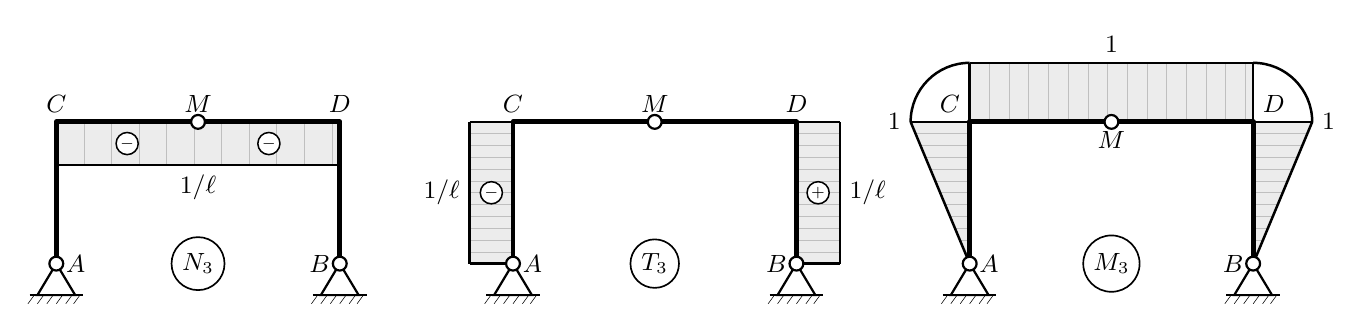
\begin{tikzpicture}[
					trave/.style={line width=1.8pt, line cap=round, line join=round, black},
					terra/.style={line width=0.8pt, black},
					diag/.style={line width=0.90pt, black},
					nodoV/.style={circle, fill=white, draw=black,
						inner sep=0pt, minimum size=5.0pt, line width=0.80pt},
					segno/.style={circle, draw=black, fill=white, inner sep=0pt,
						minimum size=8pt, font=\tiny, line width=0.55pt},
					etlab/.style={circle, draw=black, line width=0.6pt,
						fill=white, inner sep=2pt, font=\small},
					lab/.style={font=\small},
					]
					
					\def\L{1.80}
					\def\SEP{5.80}
					\def\dNt{0.55}   % N₃ traverso: 1/ℓ → 0.55 cm
					\def\dTt{0.55}   % T₃ montanti: 1/ℓ → 0.55 cm
					\def\dMt{0.75}   % M₃: M=1 → 0.75 cm
					
					\def\portale{\draw[trave](0,0)--(0,\L)--(2*\L,\L)--(2*\L,0);}
					\def\cernieraA{%
						\draw[terra](0,0)--(-0.24,-0.40)--(0.24,-0.40)--cycle;
						\draw[terra](-0.34,-0.40)--(0.34,-0.40);
						\foreach \x in {-0.28,-0.16,-0.04,0.08,0.20,0.30}
						\draw[very thin](\x,-0.40)--++(-0.08,-0.11);
						\node[nodoV]at(0,0){};}
					\def\cernieraB{%
						\draw[terra](2*\L,0)--(2*\L-0.24,-0.40)--(2*\L+0.24,-0.40)--cycle;
						\draw[terra]({2*\L-0.34},-0.40)--({2*\L+0.34},-0.40);
						\foreach \x in {-0.28,-0.16,-0.04,0.08,0.20,0.30}
						\draw[very thin]({2*\L+\x},-0.40)--++(-0.08,-0.11);
						\node[nodoV]at(2*\L,0){};}
					
					%%═══ PANNELLO (a) — N₃ ═════════════════════════════════════════════════
					%% N = 0 sui montanti, compressione 1/ℓ uniforme sul traverso (sotto)
					\begin{scope}[xshift=0cm]
						\fill[gray!15](0,{\L-\dNt})--(2*\L,{\L-\dNt})--(2*\L,\L)--(0,\L)--cycle;
						\foreach \x in {0.35,0.70,...,3.50}
						{\draw[gray!50,very thin](\x,{\L-\dNt})--(\x,\L);}
						\draw[diag](0,{\L-\dNt})--(2*\L,{\L-\dNt});
						\portale \cernieraA \cernieraB
						\node[nodoV]at(\L,\L){};
						\node[segno]at({0.5*\L},{\L-\dNt/2}){$-$};
						\node[segno]at({1.5*\L},{\L-\dNt/2}){$-$};
						\node[below=0.04,lab]at(\L,{\L-\dNt}){$1/\ell$};
						\node[right,lab]at(0,0){$A$};
						\node[left,lab]at(2*\L,0){$B$};
						\node[above,lab]at(0,\L){$C$};
						\node[above,lab]at(2*\L,\L){$D$};
						\node[above,lab]at(\L,\L){$M$};
						\node[etlab]at(\L,{0}){$N_3$};
					\end{scope}
					
					%%═══ PANNELLO (b) — T₃ ═════════════════════════════════════════════════
					%% T negativo su AC (esterno=sinistra), positivo su BD (esterno=destra), nullo sul traverso
					\begin{scope}[xshift=\SEP cm]
						%% T montante sinistro (negativo, esterno = sinistra)
						\fill[gray!15]({-\dTt},0)--(0,0)--(0,\L)--({-\dTt},\L)--cycle;
						\foreach \y in {0.15,0.30,...,1.75}
						{\draw[gray!50,very thin]({-\dTt},\y)--(0,\y);}
						\draw[diag]({-\dTt},0)--({-\dTt},\L);
						\draw[diag]({-\dTt},0)--(0,0);
						\draw[diag]({-\dTt},\L)--(0,\L);
						%% T montante destro (positivo, esterno = destra)
						\fill[gray!15](2*\L,0)--({2*\L+\dTt},0)--({2*\L+\dTt},\L)--(2*\L,\L)--cycle;
						\foreach \y in {0.15,0.30,...,1.75}
						{\draw[gray!50,very thin](2*\L,\y)--({2*\L+\dTt},\y);}
						\draw[diag]({2*\L+\dTt},0)--({2*\L+\dTt},\L);
						\draw[diag](2*\L,0)--({2*\L+\dTt},0);
						\draw[diag](2*\L,\L)--({2*\L+\dTt},\L);
						\portale \cernieraA \cernieraB
						\node[nodoV]at(\L,\L){};
						\node[segno]at({-\dTt/2},{\L*0.50}){$-$};
						\node[segno]at({2*\L+\dTt/2},{\L*0.50}){$+$};
						\node[left=0.04,lab]at({-\dTt},{\L*0.50}){$1/\ell$};
						\node[right=0.04,lab]at({2*\L+\dTt},{\L*0.50}){$1/\ell$};
						\node[right,lab]at(0,0){$A$};
						\node[left,lab]at(2*\L,0){$B$};
						\node[above,lab]at(0,\L){$C$};
						\node[above,lab]at(2*\L,\L){$D$};
						\node[above,lab]at(\L,\L){$M$};
						\node[etlab]at(\L,{0}){$T_3$};
					\end{scope}
					
					%%═══ PANNELLO (c) — M₃ ═════════════════════════════════════════════════
					%% M lineare sui montanti (0 in A/B, 1 in C/D, entrambi verso l'esterno)
					%% M uniforme sul traverso (valore 1, sopra = lato teso)
					\begin{scope}[xshift={2*\SEP cm}]
						%% M montante sinistro (triangolo a sinistra: 0 in A, 1 in C)
						\fill[gray!15](0,0)--(-\dMt,\L)--(0,\L)--cycle;
						\begin{scope}
							\clip(0,0)--(-\dMt,\L)--(0,\L)--cycle;
							\foreach \y in {0.15,0.30,...,1.75}
							{\draw[gray!50,very thin]({-\dMt-0.1},\y)--(0.1,\y);}
						\end{scope}
						\draw[diag](0,0)--(-\dMt,\L);
						\draw[diag](-\dMt,\L)--(0,\L);
						%% M montante destro (triangolo a destra: 0 in B, 1 in D)
						\fill[gray!15](2*\L,0)--({2*\L+\dMt},\L)--(2*\L,\L)--cycle;
						\begin{scope}
							\clip(2*\L,0)--({2*\L+\dMt},\L)--(2*\L,\L)--cycle;
							\foreach \y in {0.15,0.30,...,1.75}
							{\draw[gray!50,very thin](2*\L-0.1,\y)--({2*\L+\dMt+0.1},\y);}
						\end{scope}
						\draw[diag](2*\L,0)--({2*\L+\dMt},\L);
						\draw[diag]({2*\L+\dMt},\L)--(2*\L,\L);
						%% M traverso (uniforme, sopra: rettangolo di altezza dMt)
						\fill[gray!15](0,\L)--(2*\L,\L)--(2*\L,{\L+\dMt})--(0,{\L+\dMt})--cycle;
						\begin{scope}
							\clip(0,\L)--(2*\L,\L)--(2*\L,{\L+\dMt})--(0,{\L+\dMt})--cycle;
							\foreach \x in {0.25,0.50,...,3.55}
							{\draw[gray!50,very thin](\x,\L)--(\x,{\L+\dMt});}
						\end{scope}
						\draw[diag](0,{\L+\dMt})--(2*\L,{\L+\dMt});   % linea superiore
						\draw[diag](0,\L)--(0,{\L+\dMt});              % chiusura sinistra (visibile)
						\draw[diag](2*\L,\L)--(2*\L,{\L+\dMt});        % chiusura destra (visibile)
						%% Archetti di continuità in C e D (stessa geometria di M₀)
						\draw[diag](-\dMt,\L) arc(180:90:\dMt);          % C: col.sin → trav
						\draw[diag](2*\L,{\L+\dMt}) arc(90:0:\dMt);      % D: trav → col.des
						%% Struttura
						\portale \cernieraA \cernieraB
						\node[nodoV]at(\L,\L){};
						%% Valori
						\node[left=0.04,lab]at(-\dMt,\L){$1$};
						\node[right=0.04,lab]at({2*\L+\dMt},\L){$1$};
						\node[above=0.04,lab]at(\L,{\L+\dMt}){$1$};
						%% Nodi
						\node[right,lab]at(0,0){$A$};
						\node[left,lab]at(2*\L,0){$B$};
						\node[above left,lab]at(0,\L){$C$};
						\node[above right,lab]at(2*\L,\L){$D$};
						\node[below=0.04,lab]at(\L,\L){$M$};
						\node[etlab]at(\L,{0}){$M_3$};
					\end{scope}
					
				\end{tikzpicture}
			}%
			\caption{Autosoluzione~$3$ ($\chi_3 = 1$, coppia unitaria in~$M$):
				diagrammi di $N_3$, $T_3$ e $M_3$ sul portale a tre cerniere.
				Gli archetti in~$C$ e ~$D$ indicano la continuità del momento flettente
				ai due nodi rigidi.}
			\label{fig:portale_autosoluzione3}
		\end{figure}
		%%%%%%%%%%%%%%%%%%%%%%%%%%%%%%%%%%%%%%%%%%%
		
		I diagrammi $N_j$, $T_j$, $M_j$ dei quattro problemi di carico
		esauriscono la fase statica dell'analisi: le incognite
		iperstatiche $\chi_1$, $\chi_2$, $\chi_3$ restano indeterminate
		fintanto che non si introduca la deformabilità della struttura
		e si impongano le condizioni di compatibilità.
		
	\end{svolgimento}
\end{esempio}

